%%%%%%%%%%%%%%%%%%%%%%%%%%%%%%%%%%%%%%%%%%%%%%%%%%%
%% LaTeX book template                           %%
%% Author:  Amber Jain (http://amberj.devio.us/) %%
%% License: ISC license                          %%
%%%%%%%%%%%%%%%%%%%%%%%%%%%%%%%%%%%%%%%%%%%%%%%%%%%

\documentclass[a4paper,11pt]{book}
\usepackage[T1]{fontenc}
\usepackage[utf8]{inputenc}
\usepackage{lmodern}
\usepackage{gensymb}
\usepackage{changepage}

%%%%%%%%%%%%%%%%%%%%%%%%%%%%%%%%%%%%%%%%%%%%%%%%%%%%%%%%%
% Title style                                           %
%%%%%%%%%%%%%%%%%%%%%%%%%%%%%%%%%%%%%%%%%%%%%%%%%%%%%%%%%

\usepackage{titlesec}

%\titlespacing\subsubsection{4pt}{12pt plus 4pt minus 2pt}{0pt plus 2pt minus 2pt}

%\titleformat{\subsubsection}[runin]{\bfseries\Large}{}{}{}[]
 
% Оновлюємо формат заголовка розділу
\titleformat{\chapter}[display]
  {\normalfont\huge\bfseries} % Стиль заголовка
  {Розділ~\thechapter}        % Формат нумерації
  {20pt}                      % Відступ
  {}

% Оновлюємо формат у змісті
%\renewcommand{\numberline}[1]{Розділ~#1\quad}
%%%%%%%%%%%%%%%%%%%%%%%%%%%%%%%%%%%%%%%%%%%%%%%%%%%%%%%%%
% Source: http://en.wikibooks.org/wiki/LaTeX/Hyperlinks %
%%%%%%%%%%%%%%%%%%%%%%%%%%%%%%%%%%%%%%%%%%%%%%%%%%%%%%%%%
\usepackage[hidelinks]{hyperref}
\hypersetup{unicode=true} % Прибирає hyperref Warning 

\usepackage[ukrainian]{babel} 

\usepackage[acronym, toc]{glossaries}

%%%%%%%%%%%%%%%%%%%%%%%%%%%%%%%%%%%%%%%%%%%%%%%%%%%%%%%%%%%%%
% Файли бібліографій                                        %
% Для кожного розділу треба додати строку:                  %
%   \addbibresource{Bibliographies/bib_<номер розділу>.bib} %
%  та відповідний файл в папці Bibliographies/              %
%  куди додавати посилання, експортовані з інших баз даних. %
%%%%%%%%%%%%%%%%%%%%%%%%%%%%%%%%%%%%%%%%%%%%%%%%%%%%%%%%%%%%%
\usepackage[backend=biber,style=numeric,natbib=true]{biblatex}
\addbibresource{Bibliographies/bib_01.bib}
\addbibresource{Bibliographies/bib_02.bib}
\addbibresource{Bibliographies/bib_03.bib}

%%%%%%%%%%%%%%%%%%%%%%%%%%%%%%%%%%%%%%%%%%%%%%%%%%%%%%%%%%%%%
% Файли зображеннь                                          %
%%%%%%%%%%%%%%%%%%%%%%%%%%%%%%%%%%%%%%%%%%%%%%%%%%%%%%%%%%%%%

\usepackage{graphicx}
\graphicspath{ {./Illustrations/} }


%%%%%%%%%%%%%%%%%%%%%%%%%%%%%%%%%%%%%%%%%%%%%%%%%%%%%%%%%%%%%
% Форматування таблиць                                      %
%%%%%%%%%%%%%%%%%%%%%%%%%%%%%%%%%%%%%%%%%%%%%%%%%%%%%%%%%%%%%
\usepackage{multirow}

%%%%%%%%%%%%%%%%%%%%%%%%%%%%%%%%%%%%%%%%%%%%%%%%
% Chapter quote at the start of chapter        %
% Source: http://tex.stackexchange.com/a/53380 %
%%%%%%%%%%%%%%%%%%%%%%%%%%%%%%%%%%%%%%%%%%%%%%%%
\makeatletter
\renewcommand{\@chapapp}{}% Not necessary...
\newenvironment{chapquote}[2][2em]
  {\setlength{\@tempdima}{#1}%
   \def\chapquote@author{#2}%
   \parshape 1 \@tempdima \dimexpr\textwidth-2\@tempdima\relax%
   \itshape}
  {\par\normalfont\hfill--\ \chapquote@author\hspace*{\@tempdima}\par\bigskip}
\makeatother

%%%%%%%%%%%%%%%%%%%%%%%%%%%%%%%%%%%%%%%%%%%%%%%%%%%
% Перша сторінка книги, що містить                %
%  - Заголовок та підзаголовок                    %
%  - Ім'я авторів                                 %
%%%%%%%%%%%%%%%%%%%%%%%%%%%%%%%%%%%%%%%%%%%%%%%%%%%

% Заголовок та підзаголовок
\title{\Huge \textbf{Лапароскопічна хірургія печінки}  
\\ \huge Ілюстрований посібник }
% Автор
%\author{\textsc{First-name Last-name}}
%\author{
%  LastName1, FirstName1
%  \and
%  LastName2, FirstName2
%  \and
%  LastName2, FirstName2
%  \and
%  LastName2, FirstName2
%}
\date{}
%%%%%%%%%%%%%%%%%%%%%%%%%%%%%
% Файл глоссарію            %
%(єдиний для всіх розділів) %
%%%%%%%%%%%%%%%%%%%%%%%%%%%%%
\makeglossaries

\newacronym{llr}{ЛРП}{Лапароскопічна резекція печінки}

\newacronym{hals}{ХАРП}{Хенд-ассистована резекція печінки}

\newacronym{hlr}{ГРП}{Гібридна резекція печінки}

\newacronym{olr}{ВРП}{Відкрита резекція печінки}

\newacronym{alr}{АРП}{Анатомічна резекція печінки}

\newacronym{non-alr}{НРП}{Неанатомічна резекція печінки}

\newacronym{llls}{ЛапЛЛС}{Лапароскопічна лівобічна латеральна секцієекомія}

\newacronym{llhe}{ЛапЛГ}{Лапароскопічна лівобічна гемегепатектомія}

\newacronym{lrhe}{ЛапПГ}{Лапароскопічна правобічна гемегепатектомія}

\newacronym{lrps}{ЛапПЗС}{Лапароскопічна правобічна задня секцієекомія}

\newacronym{lras}{ЛапППС}{Лапароскопічна правобічна передня секцієекомія}

\newacronym{lmhe}{ЛапМГЕ}{Лапароскопічна мезогепатектомія}

\newacronym{lce}{ЛапКЕ}{Лапароскопічна каудальна лобектомія}

\newacronym{flr}{МПЗ}{Майбутній печінковий залишок}

\newacronym{bclc}{BCLC}{Barcelona clinic liver cancer staging}

\newacronym{NCCN}{NCCN}{National Comprehensive Cancer Network}

\newacronym{alpps}{ALPPS}{Associating Liver Partition and Portal Vein Ligation for Staged Hepatectomy}

\newacronym{cvp}{ЦВТ}{Центральний венозний тиск}

\newacronym{pdl}{ПДЗ}{Печінково-дванадцятиперсна зв'язка}

\newacronym{ivc}{НПВ}{Нижня порожниста вена}

\newacronym{hv}{ПВ}{Печінкові вени}

\newacronym{lhv}{ЛПВ}{Ліва печінкова вена}

\newacronym{mhv}{СПВ}{Серединна печінкова вена}

\newacronym{rhv}{ППВ}{Права печінкова вена}

\newacronym{hcc}{ГЦК}{Гепатоцеллюлярна карцинома}

\newacronym{crlm}{МКРП}{Метастази колоректального раку в печінку}

\newacronym{nelm}{МНЕП}{Метастази нейроендокринних пухлин в печінку}

\newacronym{btc}{РБТ}{Рак біліарного тракту}

\newacronym{ihcc}{ВПХК}{Внутрішньопечінкова холангіокарцинома}

\newacronym{phcc}{ПХК}{Перихіларна холангіокарцинома}

\newacronym{gbc}{РЖМ}{Рак жовчного міхура}

\newacronym{blt}{ДПП}{Доброякісні пухлини печінки}

\newacronym{hca}{ГЦА}{Гепатоцелюлярна аденома}

\newacronym{fnh}{ФНГ}{Фокальна нодулярна гіперплазія}

\newacronym{hmg}{ГП}{Гемангіома печінки}

\newacronym{bca}{БЦА}{Біліарна цистаденома}

\newacronym{pil}{ПВХ}{Первинний внутрішньопечінковий холелітіаз}

\newacronym{ct}{СКТ}{Спіральна комп'ютерна томографія}

\newacronym{us}{УЗД}{Ультразвукове дослідження}

\newacronym{mri}{МРТ}{Магнітно-резонансна томографія}

\newacronym{icg}{ICG}{Індоціанін зелений}





%%%%%%%%%%%%%%%%%%%%%%%%%%%%%
% Основна частина документа %
%%%%%%%%%%%%%%%%%%%%%%%%%%%%%
\begin{document}

%%%%%%%%%%%%%%%%%%%%%%%%%%%%%%%%%%%%%
%       Шрифти з кирилицею          %
%%%%%%%%%%%%%%%%%%%%%%%%%%%%%%%%%%%%%

\usefont{T2A}{fcm}{m}{n} % ++++
%\usefont{T2A}{cmr}{m}{n} % ++++
%\usefont{T2A}{ftm}{m}{n} % -----
%\usefont{T2A}{PTSerif-TLF}{m}{n} % --
%\usefont{T2A}{PTSans-TLF}{m}{n} % +-
%\usefont{T2A}{cmss}{m}{n} % ---
%\usefont{T2A}{antt}{m}{n} % +-
%\usefont{T2A}{Tempora-TLF}{m}{n}



\frontmatter
\maketitle

\newpage

Сучасна хірургія печінки зазнала значних змін завдяки розвитку мінімально інвазивних технологій. Історично, лапароскопічна хірургія розвивалася протягом останніх кількох десятиліть, починаючи з перших експериментальних операцій, які часто супроводжувалися високими ризиками та невизначеністю. Проте, завдяки наполегливій праці хірургів та інженерів, ця методика стала стандартом у провідних клініках світу. Лапароскопічні резекції печінки, які ще двадцять років тому здавалися технічно неможливими, сьогодні вважаються золотим стандартом лікування. Ця трансформація не лише зменшила травматичність операцій, але й значно покращила післяопераційне відновлення пацієнтів, що є критично важливим аспектом у хірургії. Важливість навчання та симуляційних технологій у підготовці нової генерації хірургів не можна переоцінити; ці інструменти дозволяють лікарям отримувати необхідні навички в безпечному середовищі. Автори цієї книги не лише детально описують технічні аспекти операцій, а й розкривають клінічні випадки, що робить книгу надзвичайно цінною для практикуючих хірургів та молодих фахівців. Це видання є унікальним внеском у навчання та практику хірургів, які прагнуть опанувати цей складний, але ефективний метод, надаючи їм необхідні знання для успішного виконання лапароскопічних втручань.

\begin{flushright}
    
\includegraphics[width=0.25\textwidth]{Illustrations/Preface/image1.png} \\
    \textit{Професор Олександр Іванович Петров}
\end{flushright}

\newpage

Видання, яке ви тримаєте в руках, є результатом багаторічного досвіду та глибокого аналізу розвитку лапароскопічної хірургії печінки. У цій книзі автори не тільки узагальнили світовий досвід, а й представили власні досягнення та інноваційні підходи. Порівняння відкритих та лапароскопічних резекцій печінки виявляє численні переваги останніх, включаючи зменшення післяопераційних ускладнень та скорочення термінів госпіталізації. Однак, існують і певні обмеження, які потрібно враховувати. Мій власний досвід впровадження лапароскопічних технологій у хірургічну практику показав, що основними викликами були не лише технічні аспекти, але й необхідність навчання команди та адаптації до нових методик. Сучасні технології, такі як 3D-візуалізація, ICG-навідна резекція та роботизована хірургія, відіграють важливу роль у покращенні безпеки втручань, дозволяючи лікарям виконувати складні операції з максимальною точністю. Ця книга стане незамінним посібником для тих, хто прагне вдосконалити свої навички у сфері сучасної гепатобіліарної хірургії, сприяючи поширенню лапароскопічних резекцій печінки серед хірургів та підвищенню якості лікування пацієнтів.

\begin{flushright}
    
\includegraphics[width=0.25\textwidth]{Illustrations/Preface/image2.png} \\
    \textit{Професор Володимир Сергійович Мельник}
\end{flushright}


%%%%%%%%%%%%%%%%%%%%%%%%%%%%%%%%%%%%%
% Auto-generated table of contents, %
%list of figures and list of tables %
%%%%%%%%%%%%%%%%%%%%%%%%%%%%%%%%%%%%%

\tableofcontents
%\listoffigures
%\listoftables

\mainmatter

\clearpage
\printglossary[type=\acronymtype,
               title=Перелік умовних позначеннь]


\begin{refsection}
\chapter{Теоретичні основи лапароскопічної хірургії печінки}

\section{Історія розвитку методики}
\subsection{Перший досвід}
Мініінвазивні втручання радикально змінили хірургічну практику за останні три десятиріччя та призвели до суттєвого покращення результатів за рахунок зменшення частоти післяопераційних ускладненнь, тривалості госпіталізації та співвідношення вартості до еффективності лікування в різних хірургічних спеціальностях, включаючи колоректальну хірургію, урологію, гінекологію та торокальну хірургію. Природньо, що зацікавленість хірургів в лапароскопічному доступі швидко розповсюдилась на гепатобіліарні втручання, спроби виконання яких в лапароскопічному варіанті було розпочато в 1987 році із першої лапароскопічної холецистектомії \cite{Litynski}. 

Для лікування уражень печінки лапароскопія була вперше впроваджена на початку 90х. Будучи широковживаною в загальній хірургії, в печінковій хірургії лапароскопія зіткнулась із багатьма перешкодами, проте переваги лапароскопічного доступу, такі як покращена візуалізація, та зменшення післяопераційних ускладненнь  надали стимул для розвитку лапароскопічних резекцій печінки (\acrshort{llr}). Перші резекції печінки в лапароскопічному варіанті були виконані в 1991 році Reich H. \cite{Reich1991a} та  в 1992 Katkhouda N. \cite{Katkhouda1992} та Gagner M. \cite{GAGNER1992}. Ці операції були крайовими резекціями невеликих, переважно доброякісних новоутворень, проте невдовзі стало зрозуміло, що результати лапароскопічних операцій порівняні із традиційними відкритими втручаннями а \acrshort{llr} є безпечним та ефективним методом лікування. Відтоді \acrshort{llr} стала потенційною альтернативою відкритій резекції печінки (\acrshort{olr}). 
На початку розвиток методики був повільним, і наступні декілька років публікації містили лише опис поодиноких випадків атипових резекцій \cite{Klotz1993, Cunningham1995}. Перша анатомічна лапароскопічна лівобічна латеральна секцієектомія(\acrshort{llls}) виконана в 1996 році \cite{Azagra1996}  відновила інтерес до \acrshort{llr} не дивлячись на те, що перші випадки анатомічних резекцій були конвертовані у відкриті втручання через масивну інтраопераційну кровотечу \cite{Hashizume1995}.  Із накопиченням досвіду покази до \acrshort{llr} були розширені до гемігепатектомій, складних сегментектомій, трисекцієектомій та навіть донорських резекцій при трансплантації печінки від живого донора \cite{Dagher2009, Cherqui2002, Jia2018}. 

\subsection{Погоджувальні конференції}

Від моменту виконання першої \acrshort{llr} кількість публікацій присвячених темі щорічно прогресивно збільшується (Рис. \ref{fig:plot1}). Стимулом до цього є посітйне вдосконалення ендохірургічного обладнання та хірургічної техніки.
Аккумуляція досвіду поставила перед хірургічною спільнотою завдання відповіді на ключові питання пов'язані з \acrshort{llr}: по-перше це безпека та відтворюваність методики а по-друге її онкологічна ефективність. Для відповіді на них та створення клінічних рекомендацій стосовно застосування \acrshort{llr} було послідовно проведено декілька погоджувальних конференцій, висновки яких відображують процес становлення лапароскопічного методу та зміну відношення до нього хірургічного загалу. 

\begin{figure}[h]
\caption{Динаміка кількості публікацій в PubMed по запиту "laparosopic liver resection" по роках}
\centering
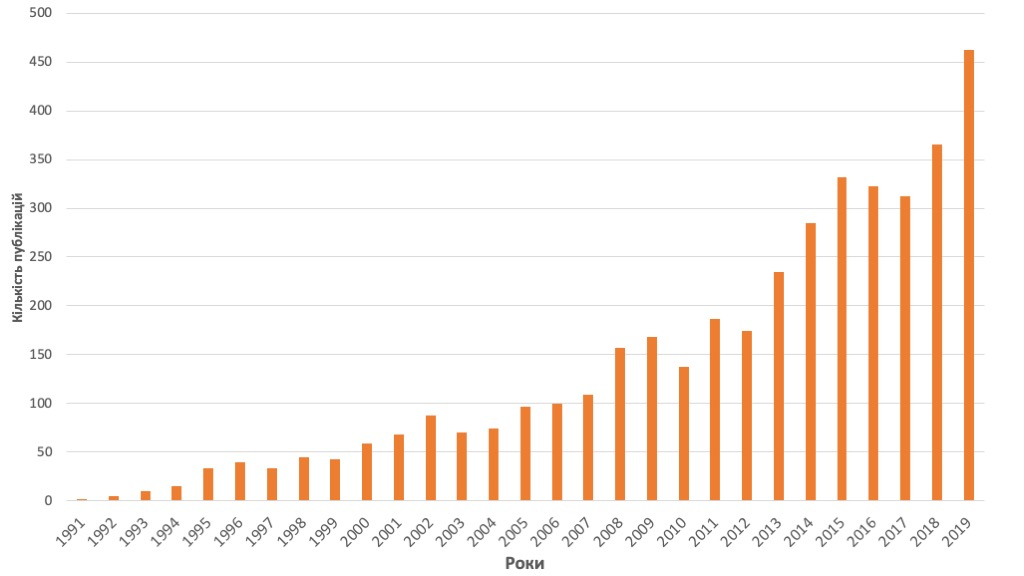
\includegraphics[width=0.9\textwidth]{Illustrations/Pic_01.jpg}
\label{fig:plot1}
\end{figure}

\subsubsection{Перша погоджувальна конференція} 

Перша погоджувальна конференція відбулась в Луізвілі в листопаді 2008 року за участі 45 міжнародних експертів з гепатобіліарної хірургії. \cite{Buell2009}. За результатами обговорення до  \acrshort{llr} були віднесені чисто лапароскопічні, хенд-асистовані резекції печінки (\acrshort{hals}) та гибридні резекції печінки (\acrshort{hlr}) при яких початкова диссекція проводиться в лапароскопічному варіанті а розсічення паренхіми через мінілапаротомію. 

Прийнятними для видалення за допомогою \acrshort{llr} були визначені утворення, розміром менше 5 см, що розташовані в 2 - 6 сегментах печінки, а \acrshort{llls} було рекомендовано розглядати в якості стандартної практики. Також була показана принципова технічна можливість видалення новоутворень, локалізованих в будь яких сегментах печінки в лапароскопічному варіанті, проте обширні резекції печінки було рекомендовано зарезервувати за спеціалізованими гепатобіліарними центрами з великим досвідом як лапароскопічних втручаннь, так і резекційної хірургії печінки. 

Конверсію рекомендовано розглядати скоріше як необхідний крок для безпечного завершення складного втручання, ніж як ускладнення. Перед ургентною конверсією з приводу кровотечі хірург повинен докласти максимальних зусиль до зупинки кровотечі лапароскопічними методами. 

Вперше була показана можливість виконання донорського забору печінки при трансплантації від живого донора у дітей в лапароскопічному варіанті. Донорську \acrshort{llls} було оцінено, як експериментальну методику, що має великий потенціал але потребує детального вивчення. 

Вцілому консенсус визначив \acrshort{llr} як безпечну альтернативу традиційним резекціям та рекомендував методику до подальшого вивчення та більш широкого впровадження досвідченими гепатобіліарними хірургами.

\subsubsection{Друга погоджувальна конференція} 

На відміну від першої, друга погоджувальна конференція, яка відбулась в японському місті Моріока в жовтні 2014 році \cite{Kaneko2015}, була побудована за Цюріхсько-Датською моделлю, та включала в себе експертну панель з 43 досвідчених хірургів та 9 членів жюрі з 18 країн які оцінювали результати \acrshort{llr}. Для оцінки були запропоновані 17 запитаннь в категоріях переваги, ризики та технічні аспекти \acrshort{llr}, відповідаючи на які жюрі сформувало рекомендації. Доказова якість рекомендацій була оцінена за шкалою GRADE а ступінь розробки втручаннь за системою IDEAL \cite{Guyatt2008, McCulloch2009}. Для об'єму резекції було запропоноване класичне визначення: до малих резекцій (Minor resection) було віднести резекції 2 та меньше сегментів а до великих або обширних (Major resection) 3 та більше сегментів. Але зважаючи на те, що технічна складність \acrshort{llls} та правобічної задньої або передньої секцієектомії в лапароскопічному варіанті значно відрізняються, резекції, до складу яких входять сегменти 7 або 8 було віднесено до великих. 

За висновками експертного жюрі як малі так і великі \acrshort{llr} не гірші за відкриті в показниках операційної летальності, післяопераційних ускладненнь, чистоті резекційного краю, загальної виживаності та вартості операції та мають перевагу в більш короткому терміні перебування в стаціонарі, меншій крововтраті. Експерти погодились з тим, що результати лапароскопічних донорських заборів не відрізнялись від відкритих у високоспеціалізованих центрах. У якості додаткового висновку жюрі заключило, що великі \acrshort{llr} вимагають високого рівню хірургічних навичок та тривалої кривої навчання.

Основними досягненнями конференції було по-перше визнання того, що  \acrshort{llr} за більшістю показників не поступаються, а за окремими показниками перевершують відкриті втручання, а по-друге рекомендація використовувати малі \acrshort{llr} в якості стандарту надання допомоги.

\subsubsection{Створення клінічних рекомендацій} 
Подальший еспотенціальний ріст кількості \acrshort{llr} призвів до того, що в лютому 2017 року в Саузхемптоні була проведена третя погоджувальна конференція \cite{AbuHilal2017a} яка мала на меті створення загальноєвропейських клінічних рекомендацій. В процесі підготовки було залучено експертну панель з 11 досвідчених гепатобіліарних хірургів, частина з яких мала досвід лише відкритих резекцій печінки а частина як відкритих так і \acrshort{llr}. Після аналітичного обзору 647 джерел, відібраних за допомогою критеріїв включення експертами були сформовані рекомендації в п'яти ключових напрямках: покази, відбір пацієнтів, види втручаннь, технічні особливості та імплементація.

Згідно з цими рекомендаціями \acrshort{llr} показані для лікування метахронних колоректальних метастазів та гепатоцеллюлярної карциноми так як ассоційовані зі зниженням крововтрати, післяопераційного асциту, печінкової недостатності та терміну перебування в стаціонарі порівняно із відкритими втручаннями при порівняній тривалості операції, частоті R0 краю резекції та рівні рецидивів. Також \acrshort{llr} показані для лікування доброякісної вогнищевої патології завдяки суттєвому зниженню післяопераційних ускладненнь, больового синдрому та терміну перебування в стаціонарі, що підтверджено на великих серіях пацієнтів, у тому числі із великими резекціями. Донорські гепатектомії наразі не є добре стандартизованими процедурами та зарезервовані за високоспеціалізованими центрами.

Що до відбору пацієнтів, то \acrshort{llr} добре показали себе у хворих з вираженою коморбідністю та можуть бути рекомендовані для пацієнтів з ожирінням та пацієнтів старшого віку. Є данні, що свідчать про полегшення перебігу повторних (відкритих або лапароскопічних) резекцій печінки у пацієнтів, що перенесли \acrshort{llr} в якості первинної операції. Складні випадки з великими новоутвореннями (> 10 см) та близкістю до магістральних судин не є протипоказами до \acrshort{llr}, так як можуть бути виконані з аналогічною відкритим операціям  морбідністю.

Усі види \acrshort{llr}, як великі так і малі, асоційовані зі зменшенням інтраопераційної крововтрати, післяопераційних ускладненнь та терміну перебування в стаціонарі та аналогічними показниками онкологічної результативності порівняно з віткритими втручаннями. Великі втручання та втручання на задніх сегментах пов'язані із більшою складністю та тривалістю операції, проте в експертних центрах можуть бути досягнуті периопераційні результати аналогічні малим \acrshort{llr}.

Також в рекомнедаціях зазначено, що жодна з існуючих технік виконання \acrshort{llr} (\acrshort{hals}, \acrshort{hlr} або чисто лапароскопічна) не показала абсолютної переваги над іншими, проте вважається, що \acrshort{hals} та \acrshort{hlr} є перехідними до чисто лапароскопічної техніки. Те ж саме стосується й техніки транссекції паренхіми: краш-кламп, використання CUSA або інших хірургічних енергій визнано рівноцінними методами. Для диссекції портальних структур більшисть хірургів використовують ізольоване лігування, проте глісоновий підхід показав аналогічні результати. Для контролю кровотечі під час \acrshort{llr} рекомендовано використовувати лапароскопічний прийом Прінгла та анастезію з низьким центральним венозним тиском (\acrshort{cvp}). Факторами ризику конверсії на відкрите втручання є високий індекс маси тіла, розмір пухлини, локалізація ураження в постеролатеральних сегментах та цирроз. Перед виконанням ургентної конверсії рекомендовано досягти тимчасового гемостаза лапароскопічними методами.

Крива навчання малих \acrshort{llr} складає 60 випадків для хірурга, що має досвід відкритих резекцій печінки. Для великих \acrshort{llr} цей показник становить 55 операцій, при умові успішного проходження кривої для малих \acrshort{llr}. Впровадження \acrshort{llr} не повинно відбуватись в ізоляції від відкритої хірургії печінки. Для кожного спелізованого гепатобіліарного центру рекомендована наявність не менше двох хірургів, спеціалізованих на \acrshort{llr}.

Якщо послідовно проаналізувати висновки всіх погоджувальних конференцій стає зрозумілим, що методика \acrshort{llr} успішно пройшла крізь етапи розробки, первинної оцінки результатів та широкого впровадження базуючись на принципах доказової медицини. Чисельна кількість дослідженнь на великих групах пацієнтів \cite{Ciria2016b, Takahara2016, Berardi2017}, в тому числі два рандомізоаних клінічних дослідження \cite{Fretland2018b, Robles-Campos2019} свідчать про перевагу \acrshort{llr} над традиційними відкритими втручаннями в періопераційних показниках зі збереженням онкологічної ефективності. 

\section[Сучасні можливості]{Сучасні можливості лапароскопічної резекційної хірургії печінки}

\subsection{Анатомічні резекції печінки}
З моменту першої \acrshort{llr} можливості методу значно поширились за межі крайових резекцій новоутворень невеликого розміру. На данний момент показана доступність виконання в лапароскопічному варіанті абсолютно всіх видів анатомічних резекцій печінки при доброякісних та онкологічних пухлинах, включно навіть з операціями при хіларній холангіокарциномі. Найбільш часто вживані резекції, такі як \acrshort{llls}, лівобічна та правобічна гемігепатектомія та моносегментектомії є добре вивченими та стандартизованими процедурами, що дозволяє деяким спеціалізованим центрам \cite{Garbarino2019} виконувати до 80-90\% всіх резекцій печінки в лапароскопічному варіанті. Тож, в більшості випадків, вибір доступу визначається скоріше можливостями клініки ніж можливостями методики. 

За об'ємом розрізняють малі (Minor) та великі або обширні (Major) резекції. До малих резекцій відносять моно- та бісегментектомії антеролатеральних сегменітв та ліву латеральну секцієектомію. До великих або обширних анатомічних \acrshort{llr} відностяь резекції при яких виляляють три або більше розташованих поруч сегмента. Класичними представниками великих резекцій є лівобічна та правобічна гемігепатектомії.

\subsubsection{Лівобічна гемігепатектомія}

Лапароскопічна лівобічна гемігепатектомія (\acrshort{llhe}) показала себе як доступна, безпечна та ефективна процедура для пацієнтів, що мають новоутворення лівої долі печінки. В ретроспективному порівняльному аналізі 62 \acrshort{llhe} та 118 відкритих лівобічних гемігепатектомій у пацієнтів з гепатоцеллюлярною карциномою (\acrshort{hcc}), внутрішньопечінковою холангіокарциномою (\acrshort{ihcc}) та деякими доброякісними новоутвореннями показано перевагу лапароскопічних втручаннь за рахунок зменшення крововтрати, часу до відновлення харчування та частоти важких ускладненнь з порівняними показниками виживаності у онкологічних хворих \cite{Cho2018b}.   Міжнародне мультицентрове ретроспективне дослідження реузльтатів 82 \acrshort{llhe} \cite{Belli2013a} не виявило достовірної різниці кількості ускладненнь та періопераційних показників у порівнянні з 222 \acrshort{llls}, - процедурою, яка є визнаним "золотим стандартом". Не дивлячись на те, що \acrshort{llhe} є технічно складнішою за \acrshort{llls}, автори рекомендують її в якості стандартного методу лікування.

\subsubsection{Правобічна гемігепатектомія}

Лапароскопічна правобічна гемігепатектомія (\acrshort{lrhe}) є непростим втручанням, так як потребує повної мобілізації та маніпуляцій з об'ємною правою долею печінки, що потребує технічної майстерності від оперуючого хірурга. З моменту першого виконання Hüscher C. в 1995 році \cite{Huscher1997} техніка \acrshort{lrhe} вдосконалювалась та зазнавала постійних модифікацій \cite{Gayet2007, Dagher2008, Homma2019, Kim2017a}. В сучасному варіанті \acrshort{lrhe} є добре вивченою процедурою. Її онкологічна еффективність та рівень ускладнень у пацієнтів з ГЦК на фоні цирозу не відрізняється від традиційної відкритої правобічної гемігепатектомії за результатами корейського моноцентрового ретроспективного псевдорандомізованого дослідження \cite{Yoon2017b}. 

\subsubsection{Секцієектомії та центральні резекції}

Окрім \acrshort{llhe} та \acrshort{lrhe} обширні резекції включають в себе праву передню, праву задню та ліву медіальну секцієектомії, мезогепатектомію. Технічно такі операції вважаються складнішими за класичні гемігепатектомії, так як включають дві площини резекції, що знаходяться під кутом одна до одної. Не дивлячись на це, в серії дослідженнь показано, що такі втручання є безпечними та відтворюваними в експертних центрах \cite{Honda2014, Cheng2015, Kim2017, Siddiqi2018}. 

\subsubsection{Складні локалізації}

Постерокраніальні сегменти (Sg 7,8) та каудальна лобектомія певний час вважались недоступними для лапароскопічного доступу через високе незручне розтажування обмежене ребрами та куполом діафрагми, та анатомічну близкість до печінкових вен та нижньої порожнистої вени (\acrshort{ivc}). В 2014 роци Ban D. та співавтори розробили шкалу складності для \acrshort{llr}, де віднесли ізольовані лапароскопічні резекції Sg 7 та 8 до резекцій вищого ступеню складності, порівняно з резекціями інших анатомічних ділянок. Для полегшення доступу до постерокраніальних сегментів Ikeda T. була запропонована напівпронована позиція пацієнта та латеральний доступ до Sg 7-8 \cite{Ikeda2014}. Пізніше Honda G. та співавторами була опублікована методика анатомичної резекції Sg 7 з внутрішньопечінковим доступом до сегментарного  гліссону \cite{Okuda2017}, а Inoue Y. показано спосіб резекції Sg 6, 7 та 8 з латерального доступу з використанням трансторакальних троакарів \cite{Inoue2017}. Описаний досвід виконання атипових резекцій печінки трансторокальним доступом при вираженому злуковому процесі в черевній порожнині \cite{Kruger2014}. Суть методу полягає в доступі до Sg 8 з правої плевральної порожнини шляхом розсічення правого куполу діафрагми.

Складність каудальної лобектомії обумовлена тим, що перший сегмент розташований в позаду печінки і безпосередньо межує з \acrshort{ivc}, що робить його пряму візуалізацію неможливою та суттєво ускладнює хірургічний доступ. Окрім того каудальна доля має власні окремі печінкові вени, які дренуються в запечінковий сегмент \acrshort{ivc}, що підвищує ризик кровотечі під час його мобілізації і робить лапароскопічну каудальну лобектомію (\acrshort{lce}) складним втручанням. В літературі є обмежені згадки про досвід виконання \acrshort{lce} переважно у вигляді кейс-репортів та невеликих серій \cite{Machado2018, Cheung2016, Koh2017, Jin2018}. Найбільшою небезпекою, пов'язаною \acrshort{lce} вважають ризик розвитку масивної неконтрольованої кровотечі з передньої стінки \acrshort{ivc} або задньої стінки серединної печінкової вени (\acrshort{mhv}), при цьому загальна морбідність складає лише 6,6\% \cite{Araki2018}. Альтернативою до лапароскопічного підходу для виконання каудальної лобектомії може стати використання роботичних систем, які полегшують маніпуляції в обмеженому просторі \cite{Marino2018a}.

\subsection[Комплексні резекції]{Комплексні резекції у поєднанні з резекцією судин чи жовчних протоків, розширеною лімфодиссекцією}

У частини пацієнтів з поширеними формами злоякісних новоутвореннь печінки спостерігається інвазія в магістральні структури печінки - ворітну вену, печінкові вени або жовчні протоки. У більшості випадків таке ураження є протипоказом до хірургічного лікування з онкологічної точки зору, проте для певної категорії пацієнтів, що страждають на локалізовані форми метастазів колоректального раку в печінку (\acrshort{crlm}) або \acrshort{hcc} чи \acrshort{phcc} хірургічне лікування у вигляді комплексної резекції печінки в комбінації із судинною або біліарною резекцією може позитивно впливати на прогноз \cite{Kobayashi2015, Tardu2016, Procopio2020, Matsukuma2020}. В більшості випадків необхідність комплексної резекції є показом до відкритого втручання, проте деякими авторами описана можливість виконання таких втручань в лапароскопічному варіанті.

\subsubsection{Резекції судин}

Огляд літератури виявив невелику кількість випадків резекцій магістральних судин виконаних під час проведення лапароскопічної резекції печінки - 3 кейс-репорти та одне дослідження серії з 6 хворих. 
Так Nomi T. та співавт. повідомляють про успішний випадок крайової резекції \acrshort{ivc} під час проведення \acrshort{lrhe} переднім доступом у 58-річного пацієнта з приводу \acrshort{crlm} \cite{Nomi2015a}. Пізніше Vega E. та співавт. виконали \acrshort{lce} з частковою резекцією \acrshort{ivc} 54-річному пацієнту, що страждав \acrshort{hcc} на фоні цирозу \cite{Vega2020}. 
Lopez-Ben та співавтори показали двохетапний лапароскопічний підхід при видаленні білобарних \acrshort{crlm} 66-річному пацієнту. Першим етапом була виконана лапароскопічна правобічна задня секцієектомія (\acrshort{lrps}) з резекцією та реконструкцією шляхом формування судинного анастомозу правої печінкової вени (\acrshort{rhv}). Під час другого етапу була виконана \acrshort{llhe}. Автори повідомляють про хороший онкологічний ефект операції та відсутність рецидивів під час огляду через 2 роки після втручання \cite{Lopez-Ben2020}.
Єдине дослідження серії випадків судинних резекцій під час проведення \acrshort{llr} належить Morise Z. та співавторам \cite{Morise2015a}. Автори заявляють про досвід 98 \acrshort{llr} з приводу \acrshort{hcc} на фоні цирозу, 6 з яких було виконано резекцію стовбура однієї з магістральних печінкових вен за допомогою лінійного степлера.
Не дивлячись на достатньо поширене застосування резекції та реконструкції стовбура ворітної вени під час виконання лапароскопічної панкреатодуоденальної резекції \cite{Kendrick2011, Garbarino2018, Wei2019} нами не було знайдено джерел, що описують застосування портопластики під час проведення \acrshort{llr}, що скоріше за все пов'язано із її технічною складністю та обмеженістю показів. 

\subsubsection{Біліарні реконструкції}

Резекція позапечінкових жовчних шляхів є обов'язковим етапом радикальних резекцій печінки з приводу \acrshort{phcc} а також може бути застосована при пухлинній інвазії іншими пухлинами. В лапароскопічному варіанті, як самостійне втручання гепатикоєюностомія широко використовується при кистах та стриктурах холедоха, як паліативне втручання, а також як частина панкреатодуоденальної резекції при пухлинах голівки підшлункової залози. Згідно доступних даних \acrshort{llr} з приводу  \acrshort{phcc} все ще є новітньою процедурою на стадії вивчення, тому досвід виконання таких операцій обмежений кейс-репортами \cite{Lin2014, Machado2014} або невеликими серіями \cite{Ratti2020}. Таким чином в експертних центрах гепатикоєюностомія є технічно доступним етапом при виконанні \acrshort{llr}, а впровадження роботичної хірургії дає надію на її більш широке застосування \cite{Machado2019, Giulianotti2010}

\subsubsection{Розширена лімфаденектомія}

Лімфодиссекція є стандартизованим етапом багатьох лапароскопічних операцій з приводу онкопатології, зокрема в мініінвазивній гінекології та хірургії шлунково-кишкового тракту \cite{Eshuis2018, Jung2019}. В резекційній хірургії печінки лімфодиссекція показана при наявності локального позапечінкового ураження лімфовузлів наприклад при \acrshort{crlm}. Не дивлячись на те, що  онкологічна ефективність привентивної лімфаденектомії при \acrshort{llr} з приводу \acrshort{ihcc} остаточно не доведена \cite{Weber2015, Zhou2019a}, багато хірургів рекомендують її рутинне виконання з метою адекватного стадіювання пухлини та визначення прогнозу \cite{Waisberg2018, Ratti2020a}.

Більшість данних про лімфаденектомію як етап \acrshort{llr} представлені у вигляді кейс-репортів та серій випадків. Їх узагальнення  наведено Levi Sandri G.B. та співавторами в оглядовій статті, на основі чого автори роблять висновок про безпечність та доступність лапароскопічного підходу \cite{Colasanti2017}. Також є результати моноцентрового псевдорандомізованого дослідження в якому Ratti F. зі співавторами порівнюють 20 пацієнтів, що перенесли \acrshort{llr} з приводу \acrshort{ihcc} із 60 аналогічними відкритими операціями. За отриманими результатами \acrshort{llr}, серед яких 85\% великих резекцій, були не гіршими від відкритих втручаннь за показниками морбідності та безрецидивної виживаності, а також були асоційовані із меншою крововтратою та більшою кількістю видалених лімфовузлів \cite{Ratti2016a}. 

\subsection{Технологія ALPPS} 

В перше технологія Associating Liver Partition and Portal vein Ligation for Staged hepatectomy(\acrshort{alpps}) була запропонована в 2011  Lang H.  \cite{Baumgart2011} в якості альтернативи звичайній двоетапній резекції печінки з лігуванням ворітної вени. Суть нововведення полягала в тому, що на першому етапі проводять санацію планованого печінкового залишку, лігування ворітного притоку  частини печінки, що видаляють та транссекція паренхіми. При цьому за рахунок потужного викиду прозапальних факторів протягом 7-14 днів відбувається швидкий приріст об'єму планованого печінкового залишку, після чого виконують другий етап, під час якого видаляють депорталізовану на першому етапі частину печінки. 

Методика привернула увагу науковців та отримала багатьох прихильників серед гепатобіліарних хірургів, як метод, що дозволяє значно розширити межі резектабельності у пацієнтів з обширними формами \acrshort{crlm} та інших пухлин завдяки інтенсивній регенерації печінкового залишку. Критики методики зазначали, що окрім переваг вона має певні недоліки, а саме високу частоту післяопераційних ускладненнь та ризики прогрессії пухлини між першим та другим етапами. 

Для подолання цих недоліків Brustia R. та співавторами було запропоновано виконувати втручання в лапароскопічному варіанті \cite{Brustia2013}. Наразі загальна кількість таких операцій не велика, що може бути пов'язано з тим, що відкрита  \acrshort{alpps} є відносно новим та методом, який досі знаходиться на етапі дослідження \cite{Melandro2019}.Так, Michal K. та співавтори \cite{Michal2020} за результатами метааналізу 23 джерел порівняли 46 мініінвазивних та 1088 відкритих \acrshort{alpps}, та дійшли до висновку, що лапароскопічні та роботичні втручання дозволяють знизити частоту ускладненнь порівняно з відкритими втручаннями та отримати більший ступінь гіпертрофії порівняно з емболізацією ворітної вени. До недоліків мініінвазивного підходу автори відносять ризик виявлення лише частини наявних вогнищ в наслідок обмеженої здатності до пальпації та складність імплементації такої процедури. 

\subsection{Лапароскопічна донорська резекція печінки} 

Трансплантація печінки від живого донора стала радикальним методом лікування дифузних захворюваннь та деяких пухлин печінки в умовах відсутності або обмеженої кількості трупних донорів. На відміну від резекцій з приводу новоутвореннь, під час виконання донорської резекції печінки перед хірургом стоять два завдання: по-перше це забезпечення безпеки та збереження здоров'я донора, по-друге забір реплантабельного та функціонального трансплантату з достатньою довжиною та придатним для пластики краєм ворітної та печінкових вен, печінкової артерії та жовчних протоків. 

Для зменшення ризику ускладненнь та раннього повернення працездатності донору в 2002 р. Cherqui D. та співавторами було запропоновано виконання донорського забору лівої латеральної секції в лапароскопічному варіанті при трансплантації дітям \cite{Cherqui2002a}. Пізніше техніка операції була адаптована та імплементована деякими центрами. Так наприклад Kim K-H. та свпіватори повідомляють про переваги лапароскопічного донорського забору лівої латеральної секції у вигляді зменшення терміну госпіталізації та пришвидшення реабілітації донора за результатами порівняння 11 таких втручаннь із 11 відкритими донорськими резекціями \cite{Kim2011}. 

Технічно більш складна донорська правобічна гемігепатектомія певний час залишалась недоступною для чисто лапароскопічного доступу. Запропоновані \acrshort{hals} та \acrshort{hlr} підходи не набули широкого розповсюдження \cite{Koffron2006, Thenappan2011, Lin2013}. Лише в 2013 р. Soubrane O. та співавторами була показана можливість донорського забору трансплантату правої долі печінки в чисто лапаропскопічному доступі \cite{Soubrane2013}. 

На теперішній момент лапароскопічний донорська гепатектомія активно застосовується більшістю великих спеціалізованих трансплантаційних центрів. Доступні результати псевдорандомізованих порівняльних дослідженнь, які демонструють переваги лапароскопічних донорських заборів над відкритими  аналогічні звичайним \acrshort{llr} при вогнищевій патології \cite{Broering2018, Park2019a}. Також показано безпеку лапароскопічного забору для реципієтнів \cite{Kwon2018a}. Йде дискуссія про стандартизацію та повсюдне впровадження методу \cite{Au2018, Samstein2018}


Таким чином за свою майже 30-річну історію \acrshort{llr} вийшла далеко за межі крайових та атипових резекцій антеролатеральних сегментів та впевнено конкурує з відкритими втручаннями у всіх галузях гепатобіліарної хірургії. 

\section{Покази до виконання лапароскопічних резекцій печінки}

Технічні можливості лапароскопічної хірургії постійно зростають а хірургічна техніка вдосконалюється завдяки чому більшість втручаннь, що раніше виконувались лише у відкритому доступі зараз можлива і в лапароскопічному варіанті. Враховуючи сучасні досягнення покази до \acrshort{llr} практично не відрізняються від показів до \acrshort{olr} - лапароскопічний досуп не обмежує хірургічні можливості, проте додає певні, властиві саме йому, особливості. 

Серед показів до резекції печінки розрізняють злоякісну та доброякісну патологію. Серед онкопатології, на долю якої приходиться 60-80\% резекцій  найбільш частими показами до хірургічного лікування є первинні пухлини печінки та жовчних шляхів, а саме гепатоцелюлярна карцинома (\acrshort{hcc}), внутрішньопечінкова (або масформуюча) холангіокарцинома (\acrshort{ihcc}), перихіларна холангіокарцинома (\acrshort{phcc}), рак жовчного міхура (\acrshort{gbc}) та метастази колоректального раку в печінку \acrshort{crlm}. 
В цьому розділі ми зосередимось на тих видах хірургічної патології печінки, при яких застосування мініінвазивного підходу дає можливість отримати позитивні результати. 

\subsection{Гепатоцеллюларна карцинома}.

Гепатоцеллюлярна карцинома (\acrshort{hcc}) є п'ятою за частотою серед причин летальності від онкологічних захворюваннь. Причиною цього є  виявлення пізніх стадій захворювання через його асимптоматичний перебіг. Поширені форми \acrshort{hcc} характеризуються судинною інвазією, яка значно утруднює їх хірургічне лікування, а також наявністю у більшості хворих супутнього хронічного захворювання печінки та цирозу які суттєво погіршують печінкову функцію. Окрім того \acrshort{hcc} є хіміорезистентною пухлиною, що робить системну хіміотерапію не ефективною.

Сучасний підхід до лікування \acrshort{hcc} базується на виборі методу лікування в залежності від стадії пухлини. Найбільш часто вживаною системою стаціювання \acrshort{hcc} є барселонська (\acrfull{bclc}, \acrshort{bclc}) \cite{Llovet2003}. Згідно \acrshort{bclc} хірургічне лікування показано на ранній та дуже ранній стадіях \acrshort{hcc}, коли пухлина представлена солітарними резектабельними вузлами, а можливми опціями лікування є етанолова або радіочастотна абляція, відкрита або лапароскопічна резекція та трансплантація печінки. 

При дуже ранній стадії \acrshort{hcc} за \acrshort{bclc} з розміром вогнища до 2 см найбільш ефективні етанолова та радіочастотна абляція  \cite{Cucchetti2013}. Пацієнтам з \acrshort{hcc} в межах міланських критеріїв та декомпенсованим цирозом печінки оптимальним методом лікування є трансплантація печінки \cite{Colombo2016}. Для всіх інших пацієнтів з резектабельними формами \acrshort{hcc} методом першого вибору є резекція печінки \cite{Heimbach2018, Kudo2011}. 

\subsubsection{Анатомічна та неанатомічна резекція} 
\acrshort{hcc} --- агресивна високоінвазивна пухлина, яка має тенденцію до ураження малих та великих внутрішньопечінкових судин, периваскулярних компартментів та жовчних шляхів. Портальні тромби спричинені судинною інвазією можуть викликати кавернозну трансформацію та перивенозну колатеральну сітку. Мікросудинна інвазія це типова особливість \acrshort{hcc}, характерна переважно менш діфференційованим пухлинам, яка підтверджує агрессивну біологію пухлини. Незалежними предикторами мікроваскулярної інвазії є розмір пухлини більший 5 см., та менший ступінь дифференціації \cite{Zimmermann2017}. Інвазія в дрібні внутрішньопечінкові гілки ворітної вени може приводити до локального ретропортального кровотоку та периферійного внутрішньопечінкового розповсюдження у вигляді числених метастатичних вузлів по ходу судин в межах портального судинного басейну локальної анатомічної ділянки \cite{Kim2008}. 

Враховуючи схильність \acrshort{hcc} до локального метастазування в межах анатомічних ділянок методом вибору хірургічного лікування є анатомічна резекція печінки (\acrshort{alr}). На відміну від неанатомічної резекції печінки (\acrshort{non-alr}) \acrshort{alr} включає в себе ідентифікацію судинного бассейну анатомічної ділянки, що містить пухлину та видалення всієї її паренхіми. Онкологічні переваги \acrshort{alr} підтверждують більшість дослідженнь, так Makuuchi M. та співавтори \cite{Shindoh2016} в дослідженні 209 пацієнтів з цирозом класу А за Чайлдом та \acrshort{hcc} розміром $\leq$ 5 см, що були резектабельні як за допомогою \acrshort{alr} так і \acrshort{non-alr} показали перевагу \acrshort{alr} завдяки меншому ризику локальних рецидивів та більшій тривалості життя. Автори метааналізу \cite{Moris2018} 43 досліджень стверджують, що у 6839 пацієнтів яким була виконана \acrshort{alr} в порівнянні з 5590 пацієнтами з \acrshort{non-alr} були кращі загальна та безрецидивна виживаність та морбідність та рання післяопераційна летальність.

До переваг \acrshort{alr} відносять кращий онкологічний ефект, а до недоліків - вищий порівняно з \acrshort{non-alr} ризик післяопераційного порушення печінкової функції, пов'язаний з більшим об'ємом резекції, що особливо важливо для пацієнтів із цирозом печінки. Враховуючи це необхідний ретельний відбір пацієнтів для резекції печінки з приводу \acrshort{hcc}, що базується на оцінці рівню печінкової недостатності, ступеню портальної гіпертензії та загального статусу пацієнта. Американські клінічні настанови National Comprehensive Cancer Network (\acrshort{NCCN}) в якості кандидатів для резекції печінки пропонують пацієнтів з компенсованою печінковою функцією, солітарним вогнищем без макросудинної інвазії та майбутнім печінковим залишком (\acrshort{flr}) $\geq$ 20\% для здорової паренхіми та $\geq$ 30-40\% з адекватним кровопостачанням та жовчевідтоком. В клінічних настановах Європейської ассоціації вивчення хвороб печінки по лікуванню \acrshort{hcc} \cite{Galle2018a} для пацієнтів з цирозом печінки запропоновано спрощений алгорим визначення ризику \acrshort{alr}, що базується на об'ємі резекції, супеню портальної гіпертензії та печінкової недостатності. 

\subsubsection{Лапароскопічна та відкрита резекція печінки при \acrshort{hcc}} 
Окрім віддалених результатів на ефективність лікування впливає післяопераційна морбідність. Першим з двох основних факторів, які впливають на післяопераційні результати під час резекції печінки з приводу \acrshort{hcc} є крововтрата. Вищий об'єм крововтрати та замісної трансфузії препаратів крові асоційований з вищою з частотою післяопераційних ускладненнь та меншою віддаленою виживаністю \cite{DeBoer2007, Romano2012}. Крововтрата викликає імунодепрессію що сприяє розвитку хірургічних інфекцій, сепсису і збільшення ризику рецидиву в подальшому. Другим фактором є післяопераційна асцитопродукція у пацієнтів з цирозом печінки, яка є грізним ускладненням, що може призводити до великих втрат білка та рідини (до 5 літрів на добу), нагноєння післяопераційної рани та погіршання печінкової функції \cite{Ishii2014}. Окрім збільшення резистивності портального русла через його зменшення внаслідок резекції печінки та набряку печінкового залишку, механізм виникнення асцитопродукції пов'язують з декомпенсацією портальної гіпертензії внаслідок переривання портосистемної колатералізації під час лапаротомії \cite{Kanazawa2013}. 

Згідно існуючих даних, лапароскопічний підхід ефективно знижує ризики обох цих ускладненнь. За рахунок більш прецизійної техніки та позитивного тиску карбоксиперитонеуму \acrshort{llr} асоційовані з меншою інтраопераційною крововтратою, а збереження цілісності колатералей передньої черевної стінки дозволяє знизити частоту та інтенсивність післяопераційної асцитопродукції \cite{Truant2011}. Також \acrshort{llr} зменшують і загальну післяопераційну морбідніть у пацієнтів з \acrshort{hcc} на фоні цирозу при вираженій портальній гіпертензії та тромбоцитопенії < 100,000/мл про що свідчать результати міжнародного мультицентрового порівняльного псевдорандомізованого дослідження результатів лікування 1974 пацієнтів \cite{Ruzzenente2020}.

\emph{Враховуючи наведене вище оптимальними показами до \acrshort{llr} при \acrshort{hcc} є резектабельні форми пухлини всіх локалізацій без ураження магістральних судин або жовчних протоків на фоні здорової паренхіми або компенсованого цирозу печінки при відсутності показів до трансплантації печінки.}

\subsection{Рак біліарного тракту}

Рак біліарного тракту (\acrshort{btc}) - гетерогенна група захворюваннь до якої відносять внутрішньопечінкову (або масформуючу) холангіокарциному (\acrshort{ihcc}), перихіларну холангіокарциному (\acrshort{phcc}), рак жовчного міхура (\acrshort{gbc}) покази до лікування яких за допомогою \acrshort{llr} будуть розглянуті нижче, та рак дистального відділу холедоха і ампулярний рак, які не відносяться до теми цієї книги. 

\subsubsection{Внутрішньопечінкова масформуюча холангіокарцинома}

\acrshort{ihcc} є другою за частотою формою первинного рака печінки з високим потенціалом диссемінації та рецидивів, що походить із клітин проксимальних гілок жовчних протоків, на долю якої припадає до 40\% первинних пухлин печінки. Резекція печінки є єдиним потенційно радикальним методом та застосовується в якості першого етапу лікування \acrshort{ihcc}. Медіана виживаності пацієнтів після радикальної резекції складає 27 - 36 міс \cite{Buettner2017}. Не дивлячись на те, що вплив лімфаденектомії на виживаність при \acrshort{ihcc} остаточно не доказано рекомнедується її рутинне виконання з метою стадіювання процесу та вибору подальшого лікування. При досягненні R0 резекцийного краю необхідна системна адьювантна хіміотерапія, яка може бути доповнена хеморадіаційними методами в разі R1 резекції або позитивних лімфовузлів. При досягненні R2 резекцийного краю із макроскопічними залишками пухлини подальше лікування пацієнта необхідно проводити згідно рекомендацій до лікування нерезектабельних форм \acrshort{ihcc}. 

Резекція печінки при \acrshort{ihcc} є комплексною процедурою, технічна складність якої посилюється лімфаденектомією та можливою резекцією позапечінкових жовчних шляхів. Не дивлячись на те, що Саузґемптонські рекомендації не визначають однозначно місце \acrshort{llr} в лікуванні \acrshort{ihcc} через обмежену кількість накопиченого досвіду внаслідок низької частоти резектабельних форм, існує кілька порівняльних дослідженнь, що свідчать на користь лапароскопічного доступу. Так, група південнокорейських авторів на основі порівняння результатів 14 \acrshort{llr} з результатами 23 \acrshort{olr} у пацієнтів з \acrshort{ihcc} зазначає, що при порівняних онкологічних результатах пацієнти, що перенесли \acrshort{llr} мали меншу крововтрату та кращі ранні післяопераційні показники \cite{Lee2016a}. Характерною особливістю дослідження є те, що в нього включені лише невеликі пухлини, розміром $\leq$ 5 см. Ці данні також підтверджує двоцентрове псевдорандомізоване дослідження групи італійських та англійських вчених, в якому на основі вивчення результатів 208 \acrshort{llr} та \acrshort{olr} автори визначають \acrshort{llr} у відібраних пацієнтів  з \acrshort{ihcc}, як доступну та онкологічно ефективну процедуру, асоційовану з меншим ризиком післяопераційних ускладненнь \cite{Ratti2020}.


\subsubsection{Перихіларна холангіокарцинома}

На відміну від інших видів \acrshort{btc}, \acrshort{phcc}, це захворювання при якому показана можливість 10-річної виживаності після хірургічного лікування на рівні 14\% при адекватному відборі пацієнтв \cite{Juntermanns2019}. Через свої біологічні особливості \acrshort{phcc} має схильність до підслизового інфільтративного росту \cite{Sakamoto1998}, що обумовлює поширення пухлини за межі макроскопічно ураження, а також до інвазії магістральних судин ще до клінічної маніфестації у вигляді механічної жовтяниці \cite{Shimada2003}. Пухлина частіше розповсюджується лімфогенним та периневральним, ніж гематогенним шляхом \cite{Zimmermann2017}. Ці морфологічні особливості визначають агресивну хірургічну тактику та об'єм  втручання при \acrshort{phcc}, яке включає резекцію печінки відповідно рівню ураження із тотальною каудальною лобектомією, резекцію позапечінкових жовчних шляхів та розширену лімфаденектомію. За необхідості втручання може бути доповнене резекцією ворітної вени та печінкової артерії при їх пухлинній інвазії а також панкреатодуоденальною резекцією при інвазії дистального края холедоха \cite{Mizuno2019}. 

Через обширність та складність втручання в літературі доступні обмежені данні про мініінвазивне оперативне лікування \acrshort{phcc}. За данними огляду літератури та метааналізу групою авторів з нідерландів у 15 джерелах загалом виявлено 142 випадки виконання радикального мініінвазивного втручання з приводу \acrshort{phcc}, з яких 82 були \acrshort{llr} і 59 робот-асистованими резекціями \cite{Mizuno2019}. Дослідження виявило, що мініінвазивний підхід дає можливість отримати післяопераційну морбідність на рівні 24\% та летальність на рівні 3\%, що порівняно з результатами відкритих резекцій, та досягнути R0 резекції у 80\%. Не зважаючи на отримані оптимістичні результати, автори досить стримані у висновках, що обумовлено недостатньою кількістю накопиченого в світі досвіду та можливістю систематичної похибки через оцінку невеликих ретельно відібраних серій випадків. 

\subsubsection{Рак жовчного міхура}

\acrshort{gbc} є найбільш агресивною формою \acrshort{btc} з медіаною виживаності без лікування 6-10 місяців \cite{Lindner2018}, що пов'язано із асимптоматичним перебігом та пізнім виявленням. Радикальне хірургічна резекція може покращити результати виживаності із досягненням медіани 32 місяців. Сучасна тактика вибору об'єму хірургічного лікування \acrshort{gbc}, зазначена в рекомендаціях \acrshort{NCCN} з лікування гепатобіліарного раку, базується на стадії захворювання та обставинах його виявлення. При аксідентальному виявленні резектабельної ранньої форми \acrshort{gbc} під час холецистектомії остання доповнюється резекцією ложа жовчного міхура печінки. При виявленні пухлини під час планової проводки гістологічного препарату на стадії T1a (без інвазії підслизового шару) рекомендовано подальше спостереження, а на стадії T1b та вище, то в залежності від об'єму інвазії в паренхіму рекомендовано виконання другим етапом резекції Sg 4a-5 печінки або правобічної трисекцієектомії з лімфаденектомією. Резекція позапечінкових жовчних шляхів виконується в залежності від наявності ураження дистального краю міхурової протоки. Виконання резекції позапечінкових жовчних шляхів з метою розширення об'єму лімфаденектомії не є виправданим.  При доопераційному виявленні \acrshort{gbc} план втручання обирається в залежності від об'єму ураження.

В рекомендаціях по лікуванню \acrshort{btc} японської спілки гепатобіліарних хірургів 2015 року зазначається, що \acrshort{gbc} є протипоказом до лапароскопічної холецистектомії у зв'язку із високим ризиком диссемінації та портових метастазів \cite{Miyazaki2015}. Проте в більш пізньому міжнародному експертному консенсусі з лапароскопічної хірургії \acrshort{gbc} 2019 року наголошується, що лапароскопічний доступ не асоційований із погіршенням виживаності при ранніх стадіях \acrshort{gbc} (Т1,Т2) не ассоційованого із гострим холециститом, якщо виконується радикальна резекція, а доведеною причиною диссемінації є пошкодження цілісності стінки жовчного міхура та видалення макропрепарату без використання контейнера. У висновках консенсуса зазначається, що незважаючи на те, що \acrshort{llr} при \acrshort{gbc} є втручанням на ранніх стадіях вивчення, вона не погіршує прогноз, а у ретельно відібраних пацієнтів може покращувати результат операції. 


\emph{Таким чином, на теперішній момент \acrshort{llr} при всіх видах \acrshort{btc} є новою перспективною методикою на етапі вивчення, тому виконання цих операцій обмежено спеціалізованими центрами гепатобіліарної хірургії з великим досвідом мініінвазивних втручаннь.}

\subsection{Метастатичні ураження печінки}

Другим за частотою після первинних пухлин печінки показом до \acrshort{llr}, є метастатичні ураження печінки. До них відносять метастази колоректального раку в печінку (\acrshort{crlm}) та метастази не колоректального походження (нейроендокринні, молочної залози та ін.)


\subsubsection{Метастази колоректального раку в печінку}

Виживаність пацієнтів з \acrshort{crlm} за останні дві декади прогресивно покращилась в результаті запровадження мультидисциплінарного підходу до лікування. Золотим стандартом лікування \acrshort{crlm} є резекція печінки, проте не дивлячись на досягнення сучасної резекційної хірургії лише 25\% пацієнтів мають резектабельні форми ураження на етапі первинної діагностики. Застосування сучасних режимів неоадьювантної хіміотерапії з урахуванням генетичного статусу дозволяє конвертувати до 40-50\% первинно нерезектабельних пацієнтів та виконати радикальну резекцію печінки та позапечінкових ураженнь із задовільною виживаністю \cite{Adam2019a}. 

При оцінці резектабельності принциповим є не кількість та локалізація ураженнь а об'єм та умови функціонування майбутнього печінкового залишку \cite{Allard2017}. Окрім того, враховуючи системну природу захворювання сама по собі пухлинна судинна інвазія не є протипоказом до хірургічного лікування, так як вона не є маркером генералізації процесу та не впливає на прогноз. У більшості випадків судини можуть бути відокремлені від пухлини або доступна судинна резекція \cite{Torzilli2017}. Враховуючи наведене вище агресивний хірургічний підхід при множинних білобарних ураженнях із ураженням магістральних судин печінки є оправданим при можливості досягнення R0 резекції.

\acrshort{llr} показали себе як ефективний метод лікування \acrshort{crlm}, що підтрержджують результати багатьох порівняльних мультицентрових та рандомізованих досліджень. Так італійське псевдорандомізоване порівняльне дослідження великої когорти пацієнтів (187 \acrshort{llr} проти 698 \acrshort{olr})  показало переваги мініінвазивних втручаннь над відкритими завдяки покращенню ранніх післяопераційних та віддалених результатів (збільшення медіани безрецидивної та загальної виживаності, менший відсоток рецидивів) \cite{Ratti2018a}. Покращена візуалізація та карбоксиперитонеум дозволяють зменшити крововтрату, що позитивно впливає на загальну кількість післяопераційних ускладненнь. Також за данними двох рандомізованих досліджень \acrshort{llr} знижує загальну запальну відповідь, що також зменшує частоту ускладненнь \cite{Kasai2018, Fretland2015}. Також на користь переваг \acrshort{llr} в показниках летальності, морбідності, чистоті резекційного краю та терміну перебування в стаціонарі свідчать результати великого рандомізованого дослідження OSLO-COMET \cite{Fretland2018a}. Окрім того \acrshort{llr} показали свою ефективність при симультантних резекціях первинного вогнища та \acrshort{crlm} \cite{Moris2019}.

Вважається, що на віддалені результати після резекції впливають скоріше біологічні властивості пухлини, ніж ширина резекційного краю. Більшість сучасних дослідників визначає R0 резекцію, як можливість досягнення резекційного краю $\geq$ 1 мм. В окремих дослідженнях показано, що R1 резекції хоча і асоційовані порівняно із R0 із вищою частотою рецидивів, проте лише незначно знижують загальну виживаність \cite{DeHaas2008}. Враховуючи це, оптимальним об'ємом хірургічного лікування \acrshort{crlm} є економні паренхімо-зберігаючі резекції \cite{Matsumura2016, Moris2017}. Використання лапароскопічного підходу для паренхімо-зберігаючих резекцій \acrshort{crlm} дає можливість досягнути до 44\% 5-річної виживаності \cite{Aghayan2018}. Також показана можливість отримання позитивних результатів від лапароскопічного доступу при виконанні двоетапних резекцій та \acrshort{ALPPS} при білобарному ураженні \acrshort{crlm} \cite{Okumura2019, Melandro2019}.

Загальний ризик рецидиву \acrshort{crlm} після резекції печінки сягає до 60\%. Моноцентрове дослідження результатів лікування 1036 пацієнтів показало, що хірургічне лікування рецидивів \acrshort{crlm} ефективне, так як  довгострокова виживаність пацієнтів після повторних резекцій порівняна з вижвиваністю після первинної резекції печінкових метастазів \cite{Wicherts2013}. Збереження максимальної кількості здорової паренїіми під час \acrshort{llr} не тільки зменшує кількість ускдадненнь, а й збільшує шанси на повторну резекцію у разі рецидиву. Також нещодавнє дослідження результатів хірургічного лікування пацієнтів з рецидивами \acrshort{crlm} показало, що повторні \acrshort{llr} асоційовані із зменшенням крововтрати та часу операції порівняно з повторними \acrshort{olr}. 

Сучасні можливості роблять доступним для лапароскопічного доступу весь спектр хірургічних втручань. \acrshort{llr} є адекватним методом лікування \acrshort{crlm}, який дозволяє досягнути кращих периопераційних результатів порівняно з \acrshort{olr}, та покращити віддалені результати у певних категорій пацієнтів. Складні процедури, такі як  двоетапні обширні резекції та \acrshort{ALPPS}, потребують проходження відповідної кривої навчання та є приорітетом спеціалізованих гепатобіліарних центрів, де є достатній досвід відкритих і лапароскопічних резекцій.

\subsubsection{Метастази нейроендокринних пухлин в печінку}

Нейроендокринні пухлини це гетерогенна група відносно рідких новоутвореннь різних органів (найчастіше кишківник, підшлункова залоза та легені), що походять із ендокринних або нервових клітин та здатні до метастазування. Резекція печінки є потенційно радикальним методом лікування метастазів нейроендокринних пухлин в печінку (\acrshort{nelm}) із 5-річною виживаністю 41-80\% при застосуванні агресивної тактики та симультантних резекцій \cite{Liu2009}. Враховуючи відносно повільний темп розвитку \acrshort{nelm}, для нерезектабельних симптоматичних форм оправданий агресивний хірургічний підхід у вигляді паліативної резекції частини уражень. Такий підхід дає можливість знизити пухлинне навантаження та симптоматику, пов'язану із гормональною гіперпродукцією, завдяки чому покращує ефективність паліативного лікування соматостатином \cite{Schmidt2014}. Також показані хороші віддалені результати трансплантації печінки із 5-річною виживаностю на рівні 67\% у окремих пацієнтів із нерезектабельними формами \acrshort{nelm} \cite{Moris2017a}.

Через рідкість патології та часті покази до обширних симультантних резекцій данні про застосування \acrshort{llr} для лікування \acrshort{nelm} обмежені. У більшості джерел представлені кейс-репорти або невеликі підгрупи у складі більш великих серій \cite{Passuello2016}. Так в нещодавньому дослідженні серії з 431 \acrshort{llr} Fuks D. та співавтори повідомляють про досягнення 70.6\% 5-річної виживаності та зниження морбідності порівняно з  \acrshort{crlm}  в гурпі з 21 \acrshort{nelm} \cite{Triantafyllidis2019}.


\subsubsection{Інші види метастатичних ураженнь}

На відміну від \acrshort{crlm} та \acrshort{nelm}, для яких резекція печінки є загальноприйнятим підходом, роль хірургії в лікуванні метастазів іншого походження досі остаточно не визначена. До цієї групи відносять широкий спектр нозологій, а саме метастази раку молочної залози, раку підшлункової залози, меланоми, пухлин наднирників, пухлин урогінекологічного походження та ін. 

Враховуючи різну природу та механізми метастазування цих захворювань результати хірургічного лікування метастазів в печінку значно відрізняються в залежності від нозології. На основі аналізу результатів лікування 1452 пацієнтів Аdam R. та співавторами була розроблена прогностична модель \cite{Adam2006}. Після мультіваріантного аналізу у якості факторів, асоційованих із поганим прогнозом автори виділили вік пацієнта $\geq$ 60 років, безрецидивний інтервал $\leq$ 12 міс., позапечінкові метастатичні ураження, R1 край резекції, великий об'єм резекції та гістологічна будова пухлини. За данними дослідження адекватна стратифікація та відбір кандидатів для резекції дозволяє досягнути 46\% 5-річної виживаності.

При наявності показів до хірургічного лікування \acrshort{llr} дає переваги у покращанні ранніх післяопераційних результатів. Це підтверждують результати нещодавнього норвезького дослідження серії з 51 лапароскопічної резекції з приводу метастатичного ураження печінки не колоректального та не нейроендокринного походження \cite{Aghayan2019}. Автори спостерігали загальну 5-річну виживаність на рівні 38\% з медіаною 37 міс. При цьому найгірші показники 5-річної виживаності (0-12\%) були у пацієнтів з метастазами адренокортикального раку та меланоми, а найкращі (49-53\%) у метастазів аденокарциноми, сквамозно-клітинної карциноми та стромальних пухлин. Автори відмічають, що  \acrshort{llr} асоційована із покращенням ранніх периопераційних показників та морбідності, аналогічно показникам при \acrshort{crlm} та \acrshort{nelm}.

\subsection{Доброякісна патологія печінки}

\subsubsection{Доброякісні пухлини печінки}

До найбільш розповсюджених доброякісних пухлин печінки (\acrshort{blt}) відносять гепатоцелюлярну аденому (\acrshort{hca}), фокальну нодулярну гіперплазію (\acrshort{fnh}), гемангіому (\acrshort{hmg}). В більшості випадків ці новоутворення є випадковими знахідками, мають невеликий розмір та не потребують хірургічного лікування, однак у частини пацієнтів вони можуть бути асоційовані із такими симптомами, як слабкість, тошнота та швидка втомлюваність, які виникають внаслідок ускладненнь (розрив, інтрамуральний крововилив) або великих розмірів новоутворення. У керівництві Європейської асоціації вивчення печінки (EASL) з лікування доброякісної патології печінки 2016 р. зазначено, що через недостатність рандомізованих досліджень які порівнюють консервативне та хірургічне лікування симптомних \acrshort{blt} роль останнього остаточно не визначена \cite{Colombo2016}. Більшість дослідників погоджуються, що при наявності у пацієнта з \acrshort{blt} абдомінальних болей, ризику малігнізації або неможливості точно встановити діагноз показана резекція печінки. Для пацієнтів з \acrshort{hca} показом до операції вважається розмір $\geq$ 5 см., так як до 25\% цих новоутворень ускладнюються кровотечею чи розривом, 5-9\% малігнізацією, а розмір пухлини прямо асоційовано із ризиком ускладненнь. Окрім розміру, показами до резекції \acrshort{hca} є чоловіча стать, наявність диспластичних вогнищ в пухлині та  β-катенін мутація через те, що ці фактори підвищують ризик малігнізації \cite{Ercolani2015}.

У пацієнтів з \acrshort{blt}, яким показано хірургічне лікування \acrshort{llr} надає переваги у зменшенні кількості та важкості ускладненнь, пришвидшенні реабілітації та покращанні якості життя порівняно із \acrshort{olr}. У ретроспективному мультицентровому європейському дослідженні результатів лікування 573 пацієнтів з \acrshort{hca} зазначається що \acrshort{llr} асоційовані із нижчими показниками морбідності ніж \acrshort{olr} та нульовою летальністю, а розмір пухлини $\geq$ 10 см. асоційований із діагнозом \acrshort{hcc} \cite{Laurent2016}. Автори метааналізу 42 досліджень до якого включено 4061 пацієнт оцінили вплив хірургічного втручання на ефективність редукції симптомів та якість життя при \acrshort{blt} зазначають, що \acrshort{llr} дозволяють знизити симптоматику у 80\% пацієнтів та асоційовані з нижчою ніж \acrshort{olr} морбідністю, частотою виникнення післяопераційних гриж та рецидивів \cite{VanRosmalen2019}. 

Щодо впливу розміру новоутворення на складність \acrshort{llr}, то результати порівняльного дослідження хірургічного лікування великих ($\geq$ 10 см) та середніх (5-9,9 см) свідчать, що лапароскопічний підхід є безпечним для пацієнтів з великими новоутвореннями, а кровотеча з пухлини не є протипоказом за умови попереднього її контролю ендоваскулярними методами \cite{McKay2020}. Окрім того, автори ще одного німецького порівняльного псевдорандомізованого з урахуванням складності втручання дослідження показали перевагу \acrshort{llr} у показниках ефективності та рекомендували при наявності показів до хірургічного лікування виконистовувати лапароскопічний підхід для всіх \acrshort{blt} незалежно від необхідного об'єму резекції.

Не дивлячись на оптимістичні результати \acrshort{llr} при \acrshort{blt} більшість міжнародних рекомендацій наголошує, що доступність лапароскопічних методик не повинна розширювати покази до хірургічного лікування цих нозологій за межі симптоматичних або з високим потенціалом малігнізації.

\subsubsection{Кістозна патологія печінки}

Найчастіше кістозні ураження печінки представлені простими ретенційними кістами та полікистозною хворобою, біліарними цистаденомами та паразитарними кістами. Більшість простих кіст асимптоматичні та не потребують лікування. При полікистозній хворобі або кістах великого розміру можлива симптоматика обумовлена компрессією суміжних органів або заміщенням паренхіми печінки. Ефективними методами лікування симптоматичних кіст є склеротерапія, лапароскопічна фенестрація, а у випадку тотального заміщення паренхіми печінки кистозною тканиною - трансплантація печінки. 

Біліарні цистаденоми (\acrshort{bca}) є епітеліальними пухлинами, що складають $\leq$ 5\% всіх кістозних уражень печінки та характеризуються повільним ростом. На відміну від простих кіст вони  мають 20-30\% потенціал малігнізації та трансформації в цистаденокарциному. \acrshort{bca} резистентні до фенестрації та аспірації, так як 50-90\% рецидивують після паліативного лікування. Радикальним методом лікування є R0 резекція, яка дозволяє досягнути низьких ($\leq$ 5\%) ризиків рецидиву та 80\% пятирічної виживаності \cite{Soares2015}. Данні щодо застосування \acrshort{llr} в хірургічному лікуванні \acrshort{bca}, які обмежені кейс-репортами \cite{Machado2014, Li2016a} та невеликими серіями \cite{Koffron2004}, свідчать, про актуальність всіх переваг лапароскопічного доступа для цієї патології.

Паразитарні кисти печінки найчастіше бувають викликані ехінококком, для якого людина є проміжним хазяїном. Симптоматика неускладненого ехінококоза як правило скудна та неспецифічна, проте при розриві чи нагноєнні кіст можуть розвиватись небезпечні для життя стани, такі як анафілактичний шок, перітоніт та септичний стан \cite{Finazzi2015}. За сучасними уявленнями лікування ехінококозу базується на комбінації протипаразитарних препаратів та черезшкірних УЗ-контрольованих втручаннь. 

При розмірі $\qeq$ 5 см та наявності біологічно активних видів кист (типи 2 та 3b за класифікацією робочої групи з ехінококозу ВООЗ) рекомендоване оперативне лікування. Хірургічні втручання при ехінококозі печінки базуються на принципі приорітету "закритих" методів (без вскриття порожнини кісти). Рекомендованими операціями є перцицистектомія або в окремих випадках резекція печінки. При їх неможливості виконують "відкриті" методи - субтотальну цистектомію або ендоцистектомію (гідатідектомію) \cite{Wen2019}. Згідно існуючого метааналізу 57 публікацій присвячених лапароскопічним методам лікування ехінококозу у 914 пацієнтів з паразитарними кистами було виконано 24(2,62\%) \acrshort{llr} які дозволили отримати радикальний ефект від лікування із задовільними післяопераційними результатами.  

Анатомічна радикальна резекція печінки є методом вибору для лікування більш агресивної форми паразитарного ураження печінки - альвеолококозу. За данними нещодавнього метааналізу \acrshort{llr} є потенційно ефективними методом лікування цього захворювання при дотриманні показів, а його результати порівняні із виконанням відкритих втручаннь \cite{Salm2019}. 

\subsubsection{Первинний внутрішньопечінковий холелітіаз}

Первинний внутрішньопечінковий холелітіаз (\acrshort{pil}) є хронічним захворюванням, більш ендемічним для східноазіатських країн, проте може зустрічатись і в європейських країнах. Захворювання може проявляти себе больовим синдромом або періодичними симптомами холангіту. Для корректного визначення способу лікування потрібно диференційювати \acrshort{pil} із вторинним холелітіазом, який може бути наслідком міграції конкрементів з жовчного міхура або наслідком попередніх гепатобіліарних втручаннь. Механізм виникниння \acrshort{pil} чітко не з'ясований, але відомо, що у європейського населення він часто асоційований з 4 типом кіст біліарного дерева (хворобою Каролі), яка є показом до трансплантації печінки. Також відомо, що \acrshort{pil} частіше локалізується в лівій долі печінки, що пов'язують із більшим кутом лівого дольового протоку до холедоху та сповільнення пасажу жовчі в ньому \cite{Giuliante2015}.

Показано хороші результати застосування \acrshort{llr} для \acrshort{pil}, особливо при найбільш частій лівобічній локалізації. Так доступні результати південнокорейського порівняльного дослідження результатів лікування \acrshort{pil}. У дослідження були включені 149 пацієнтів із \acrshort{pil}, яким було виконано резекцію печінки відкритим та лапароскопічним шляхом, на основі аналізу результатів лікування яких автори дійшли висновку, що \acrshort{llr} є радикальним та безпечним методом лікування, який дозволяє знизити післяопераційну морбідність та асоційований із скороченням періоду реабілітації.

\section{Лапароскопічний погляд на хірургічну анатомію печінки}

Лапароскопічна хірургія має відмінності у візуалізації порівняно із відкритою хірургією, які пов'язані із відображенням плоскої, спотворенної заломленням світла при проходженні крізь оптичну частину лапароскопа проекції тривимірного зображення на екран. Такі відмінності зумовлюють особливий вигляд анатомічних структур та затруднюють їх ідентифікацію відносно звичних орієнтирів. Розуміння принципів виникнення таких особливостей є основою для безпечного виконання \acrshort{llr}. У цьому підрозділі ми розглянемо сучасні погляди на анатомічну будову печінки та особливості її лапароскопічної візуалізації.

\subsection{Сучасна номенклатура хірургічної анатомії печінки}

Резекційна хірургія печінки в теперішньому вигляді не була б можливою без детального уявлення про її внутішню анатомічну будову. Сучасні знання про анатомію печінки базуються на работах Healey J., Schroy P. і Couinaud С., які розробили принципи сегментарного поділу печінки. В класифікації Couinaud С., печінка поділяється на ліву та праву напів-печінку, кожна з яких в свою чергу ділеться на медіальний та латеральний сектори по ходу лівої та правої печінкових вен \cite{COUINAUD1954}. Кожен з секторів, окрім лівого латерального далі поділяється на два сегменти. Першим сегментом (Sg I) печінки є каудальна доля, яка має автономне кровопостачання. Враховуючи каудальну долю загальна кількість сегментів по Couinaud складає 8 (у більш пізній версії класифікації автор виділив хвостатий відросток Sg I у окремий 9-й сегмент) і вони мають нумерацію по ходу годинної стрілки за анологією з районами Парижу. Кожен сегмент за Couinaud - це ділянка паренхіми печінки, яка має автономне кровопостачання та жовчовідтік за рахунок гілок глісонів третього порядку. 

Класифікація Healey J. та Schroy P. використовує подібний принцип поділу, але на відміну від класифікації Couinaud поділяє печінку на ліву та праву долі, що діляться на сегменти (аналог секторів за Couinaud), які в свою чергу діляться на ділянки (аналог сегментів за Couinaud) \cite{HEALEY1953}. Принципово в цих двох класифікаціях відрізняється принцип поділу лівої долі печінки, яку Couinaud поділяє на сектори за ходом ворітної вени (до медіального сектору віднесено Sg 3, 4 а до латерального -  Sg 2), а Healey на сегменти за ходом жовчних шляхів та печінковї артерії (до медіального сегменту віднесено Sg 4 а до латерального - Sg 2,3).  

Так, як обидві класифікації мають широке розповсюдження в світі, з метою стандартизації на погоджувальній конференції в Брісбані у 2000 році Міжнародною Гепатопанкреатобіліарною Асоціацією було запропоновано універсальну номенклатуру для визначення анатомічних областей та видів резекцій печінки \cite{Pang2000}. Брисбанська класифікація побудована на основі класифікації Couinaud із заміною терміну "сектор" на "секція", за виключенням будови лівої долі, де Sg 2,3 віднесені до лівої латеральної секції. Згідно цієї класифікації таким анатомічним зонам, як напів-печінка (доля), секція та сегмент відповідають операції гемігепатектомія, секцієектомія та сегментектомія. Для уникнення термінологічних розбіжностей у цьому виданні ми будемо користуватись виключно номенклатурними термінами відповідно Брісбанській класифікації 2000 року.

\subsection{Лапароскопічна візуалізація зовнішніх орієнтирів}

На геометрію лапароскопічного зображення впливають кут огляду, кут напрямку зору та відстань до об'єкту. Скошена оптика (із кутом напрямку зору 30 та 45 градусів) дозволяє зробити огляд з різних боків, проте має більший ступінь спотворення зображення. Окрім того обмежений робочий простір, створений карбоксиперитонеумом, робить утрудненою візуалізацію цілого органу.

\subsubsection{Зв'язковий апарат}

Печінка вкрита очеревиною зі всіх боків, окрім невеликої частини  де очеревина переходить на діафрагму та формує коронарну зв'язку, яка далі переходить в ліву та праву трикутні зв'язки які разом утворюють її фіксуючий апарат. Серповидна зв'язка йде сагітально по серединній лінії від пупка та містить круглу зв'язку в свому вільному краї. Кругла зв'язка прямує до умбілікальної фіссури по вісцеральній поверхні лівої долі печінки, де входить в печінку та закінчується облітерованою частиною умбілікальної порції лівої ворітної вени. 

Серповидна зв'язка є чітким лапароскопічним орієнтиром, що відмежовує ліву латеральну секцію від інших сегментів печінки. Ліва трикутна зв'язка повністю доступна огляду по задньому краю Sg 2 печінки. Для візуалізації нижнього краю правої трикутної зв'язки необхідно підняти праву долю печінки. Верхній край правої трикутної зв'язки майже не доступний візуалізації без попередньої мобілізації її нижнього краю та коронарної зв'язки.

\subsubsection{Структури печінково-дванадцятиперсної зв'язки}

В складі печінково-дванадцятиперсної зв'язки (\acrshort{pdl}) в печінку входять ворітна вена, печінкова артерія, гілки блукаючого нерва, а виходять жовчні та лімфатичні протоки. Структури \acrshort{pdl} покриті жировою та сполучною тканиною і шаром очеревини, яка переходить в малий сальник по лівому краю зв'язки. Пряма лапароскопічна візуалізація структур \acrshort{pdl} без диссекції можлива лише частково, як правило у пацієнтів з малою кількістю абдомінального жиру. Зовнішніми орієнтирами є шийка жовчного міхура, отвір Вінслоу та малий сальник. Після холецистектомії сають доступними до візуалізації проекції правих переднього та заднього глісонів та глісону каудального відростку Sg 1. 
\subsection{Капсула Лаенека та концепція «вхідних воріт» для глісонового підходу}

Вперше описана Laennec в 1802 р. власна капсула печінки є тонкою мембраною, яка лежить субсерозно та на відміну від очеревини покриває цілий орган. Пізніше Couinaud була сформована концепція Глісонового плато - потовщеної фіброзної пластини, яка покриває судинно секреторні структури в складі Глісонових ніжок. Плато умовно ділять на три частини - хіларне, умбілікальне та міхурове, які переходять одне в інше. Також на основі гістологічних досліджень він довів, що капсула Лаенека не продовжується на Глісонові ніжки в складі хіларного плато, а йде окремим шаром вздовж усіх глісонових структур та печінкових вен, що входять в паренхіму печінки.

За сучасними уявленнями капсула Лаенека йде паралельно до глісонових структур, але в деякіх ділянках не прилягає до них щільно. Ця особливсість дає можливість безпечного хірургічного підходу до позапечінкового виділення Глісонових структур під час \acrshort{alr}, тому простір в місцях нещільного прилягання капсули Лаенека до глісонових гілок має назву "вхідних воріт". Всього виділяють шість вхідних воріт для визначення яких є чотири анатомічних орієнтира - Аранцієва протока, умбілікальне плато, міхурове плато та Глісонова ніжка каудального відростка. Межею I воріт є каудальний кінець Аранцієвої протоки, II воріт - з'єднання між круглою зв'язкою та умбілікальним плато, III воріт - правий край лівого дольового глісону (Sg 2-4), IV воріт - лівий край правого переднього глісону, V воріт - біфуркація правих сегментарних глісонів, а VI воріт - простір між краєм заднього глісону та глісоном каудального відростку. 

Диссекція в цих анатомічних ділянках та послідовне з'єднання між собою сусідніх воріт дозволяє виконати позапечінкову ізоляцію будь якого глісону з метою наступного виконання анатомічної резекції. Усі вхідні ворота легко доступні для лапароскопичноъ візуалізації: ворота I - III безпосередньо, а ворота IV - VI після попередньої холецистектомії (мал №)

\subsection{Анатомічна будова Sg I печінки}

Перший сегмент печінки або каудальна доля це центродорзально розташована ділянка паренхіми, яка має незалежне кровопостачання та жовчевідтік. Анатомічно вона обмежена наступними структурами: по задньому краю запечінковим сегментом \acrshort{ivc}, по нижньому краю воротами печінки, по верхньому - устям правої та загальним устям лівої та серединної печінкових вен, по пердньому та правому краю - тканиною Sg 4-8, а по лівому має зовнішню поверхню, вкриту капсулою (Спігелєва доля), яка пролабує до малого сальника та обмежена Аранцієвим протоком. Відповідно до класифікації Kumon M. \cite{Kumon2017}, каудальна доля поділяється на три частини: 1) Спігелєва порція (доля),  2) Паракавальна порція, 3) Порція каудального відростка. Для прямої лапароскопічної візуалізації  доступна лише частина каудального відростка та спігелєва доля після розсічення малого сальника.

Каудальна доля має власні портальні гілки, які йдуть від біфуркації ворітної вени в дорзальному напрямку. Аналогічно до портальних гілок, каудальна доля має власні артеріальні гілки від лівої та правої печінкових артерій та жовчні протоки, що дренуються в області конфлюенся лівого та правого дольових жовчних протоків. Спігєлева доля та порція каудального відростка мають по одній власній печінковій вені а паракавальна порція - декілька коротких печінкових вен, які дренуються безпосередньо в \acrshort{ivc}. 


\subsubsection{Нижня порожниста вена та печінкові вени}

Запечінковий сегмент \acrshort{ivc} інтимно прилягає до Sg 1 печінки звідки в нього дренуються короткі печінкові вени та обмежений згори окремим устям правої та загальним устям лівої та серединної печінкових вен. Для повної лапароскопічної візуалізації \acrshort{ivc} необхідна мобілізація правої коронарної зв'язки та пересічення коротких печінкових вен. 

\printbibliography[heading=subbibliography] 

\end{refsection}  
\chapter{Практичні аспекти лапароскопічних резекцій печінки}
\begin{refsection}

\section{Обстеження та передопераційна підготовка пацієнтів}

\subsection{Передопераційне обстеження}

Передопераційне обстеження пацієнтів з попередньо встановленим діагнозом, що плануються на \acrshort{llr} має вирішувати дві основіні клінічні задачі: 1) планування об'єму втручання та 2) виявлення можливих протипоказів до операції та супутніх захворюваннь. 

До дослідженнь, які вирішують задачу верифікації діагнозу та планування операції відносять:
\begin{itemize}
  
  \item \textbf{Контраст-підсилена спіральна комп'ютерна томографія (\acrshort{ct}) черевної порожнини та грудної клітини} -- основний метод візуалізації новоутвореннь печінки, який дозволяє оцінити локалізацію ураження, взаємовідношення його до магістральних внутрішньопечінкових структур і анатомічні особливості кровопостачання органа. За допомогою \acrshort{ct}-волюметрії оцінюють розміри потенційного печінкового залишку, що дозволяє обрати об'єм резекції. 
  
  \item \textbf{Контраст-підсилена магнітно-резонансна томографія (\acrshort{mri}) печінки з режимом зваженої дифузії та холангіографією} -- ефективний метод дифференційної діагностики, що дозволяє ідентифікувати вогнища невеликого розміру. \acrshort{mri}-холангіографія є неінвазивним способом отриманя інформації про взаємовідношення новоутворення печінки до жовчних шляхів. Найчастіше \acrshort{mri} використовується в комбінації з \acrshort{ct} так як методи доповнюють один інший. 
  
  \item \textbf{Ультразвукове дослідження (\acrshort{us}) черевної порожнини} використовують як допоміжний метод візуалізації а також функціональної оцінки вісцерального кровотоку в Допплер-режимі. Інтраопераційний (\acrshort{us}) дозволяє візуалізувати новоутворення розташовані глибоко в паренхімі.
  
  \item \textbf{Лабораторні тести.} Інтегральним маркером  стану печінки є розгорнутий біохімічний аналіз крові. Оцінити його можна за допомогою шкал MELD та Child-Pugh. Стадіювання за цими системами дає можливість оцінити ризики післяопераційної печінкової недостатності у пацієнтів що мають супутнє дифузне захворювання печінки (наприклад цироз або синдром обструкції синусоїдів).
  
  \item \textbf{Функціональна проба з індоціаніном зеленим \acrshort{icg}}. \acrshort{icg} є речовиною що виводиться з організму виключно через жовч. Визначення концентрації \acrshort{icg} на 15 хвилині після введення дозволяє оцінити екскреторну функцію печінки. Наявність більше ніж 10\% від початкової концентрації говорить про порушення функції печінки.
  
  \item \textbf{Вимірювання градієнту тиску заклинювання печінкових вен (для пацієнтів з портальною гіпертензією)} є інвазивним ендоваскулярним методом прямої оцінки портального тиску. При цьому дослідженні манометром під'єднаним до  ангіохірургічного катетера вимірюється різниця тисків між вільним положенням в \acrshort{ivc} та заклиненим положенням в гілку печінкової вени. Підвищення цієї різниці тисків вище 10 мм.рт.ст свідчить про наявність вираженої портальної гіпертензії.

\end{itemize}

Для виявлення супутньої патології та можливих протипоказів виконують:

\begin{itemize}
  \item розширені загальний та біохімічний аналізи крові, коагулограмма, загальний аналіз сечі
  \item гастро- та колоноскопія
  \item УЗД черевної порожнини
  \item Електрокардіографія, Ехокардіографія
  \item Консультації суміжних спеціалістів за наявності показів (кардіолог, гінеколог/уролог, судинний хірург та ін.) 
\end{itemize}

Наведений перелік обстеженнь є базовим, та за необхідності може бути розширений додатковими дослідженнями. 

\subsection{Відомі протипокази}

Протипокази до \acrshort{llr} можна умовно поділити на абсолютні та відносні. 

До \textbf{абсолютних} протипоказів відносять явища нестабільної гемодинаміки (обумовлені наприклад септичним станом пацієнта) та відсутність толерантності до карбоксиперитонеуму внаслідок серцево-судинної недостатності. Такі стани є загрозливими для життя та як правило потребують попередньої коррекції. При наявності життєвих показів до оперативного лікування у таких хворих перевага повинна надаватись відкритим втручанням. 

\textbf{Відносними} протипоказами до виконання резекції печінки в лапароскопічному варіанті є: 
\begin{itemize}
  \item \textit{Стан після перенесеного перитоніту.} Сама по собі наявність попереднього втручання не є протипоказом до \acrshort{llr}, так як в більшості випадків лапароскопічних засобів достатньо для вісцеролізу. Проте виражені запальні процеси в черевній порожнині можуть призводити до формування щільних злук по типу "панциря", що значно утруднює операцію.
  
  \item \textit{Наявність великої пухлини або гепатомегалія.} Це потребує прикладання до органу більшої фізичної сили, що може призводити до їх розривів та кровотеч. Критичним для прийняття рішення є не абсолютний розмір пухлини, а його відношення до об'єму вільної черевної порожнини.
  
  \item \textit{Інвазія пухлини в оточуючі органи, яка потребує їх резекції.} Наявність процесу такої розповсюдженності значно збільшує об'єм та складність резекції. 
  
  \item \textit{Інвазія пухини в магістральні внутрішньопечінкові судини та жовчні протоки, що потребує їх реконструкції.} Такі втручання можливі в лапароскопічному варіанті, але пов'язані із високою технічною складністю, крововтратою та тривалим часом операції.
  
\end{itemize}

При наявності у хворого відносних протипоказів рішення про виконання операції в відкритому або лапароскопічному варіанті повинно базуватись на оцінці співвідношення потенційних ризиків та користі для пацієнта в кожному конкретному випадку. 

\subsection{Безпосередня підготовка до втручання}

Підготовка до \acrshort{llr} не відрізняється від підготовки до аналогічного відкритого втручання та включає:
\begin{itemize}
    \item отримання згоди на операцію пацієнта або особи, що представляє його інтереси після отримання ними вичерпної інформації про заплановане лікування
    
    \item обмеження прийому їжі з 18 годин попередньої доби
    
    \item обмеження прийому рідини за 6 годин до операції
    
    \item підготовка шкіри шляхом зістригання волосся за допомогою тримера
    
    \item підготовка кішківника шляхом очисних клізм або прийому послаблювальних засобів на основі макрогола
    
    \item зупинки прийому антикоагулянтів та антиагрегантів за 7-10 днів до втручання (після погодження із профільними спеціалістами)
\end{itemize}



\section{Технічне забезпечення лапароскопічних резекцій печінки}

\subsection{Вимоги до лапароскопічної стійки}

\subsection{Інструменти доступу та видалення препарату}

\subsection{Базові інструменти}

\subsection{Зшиваючі аппарати}

\subsection{Хірургічні енергії}

\subsection{Спеціалізоване обладнання}


\section{Етапи лапароскопічної резекції печінки}

\subsection{Укладка пацієнта}

В лапароскопічній хірургії положення пацієнта є ключовим фактором, який впливає на ефективність операції. В умовах, коли тракція органів обмежена можливостями ендоінструментів та об'ємом замкнутої черевної порожнини, позиціонування пацієнта може, за рахунок гравітації, забезпечити необхідну експозицію. Окрім початкової позиції на столі важлива динамічна адаптація нахилу самого хірургічного стола відповідно завданням кожного з етапів втручання. Через значний вплив на технічну складову операції ми вважаємо за доцільне розглядати укладку пацієнта як один з етапів \acrshort{llr}.

\subsubsection{Загальні принципи укладки пацієнта}

Позиція пацієнта повинна відповідати запланованому втручанню та анатомічним особливостям пацієнта. Вибір позиції обумовлює запланована лінія транссекції, яка в оптимальному варіанті повинна знаходитись безпосередньо перед хірургом, в продовженні фізіологічної площини його зору. 

Нахил столу повинен забезпечувати основну гравітаційну тракцію внутрішніх органів, яку хірург лише моделює ендоінтструментами. Такий підхід значно знижує ризик травматичних пошкодженнь. Як правило, після постановки портів стіл переводять в зворотнє положення Транделенбурга, що дозволяє відвести кішківник в нижні відділи черевної порожнини. За потреби ця позиція може бути доповнена ізольованим опущенням головного кінця столу. При цьому необхідно щоб положення попереку пацієнта співпадало по рівню з відповідним шарнірним механізмом столу. Нахил столу вліво чи вправо повинен постійно змінюватись в залежності від потреб поточного етапу операції. 
Анестезіологічна бригада повинна бути попереджена про постіну необхідність таких змін положення операційного столу, так як це може впливати на розташування обладнання. 

Після укладки пацієнт повинен бути прифіксований до столу спеціальними ременями, що йдуть в комплекті. Для профілактики позиційних плекситів необхідно намагатись забезпечити максимально можливе фізіологічне положення кінцівок. Перед накриттям пацієнта стерильною білизною необхідно перевірити можливі місця прилягання до тіла пацієнта твердих деталей столу та захистити ці місця силіконовими подушками з метою попередження утворення пролежнів. Також треба уникати можливого провисання попереку та плеча при латеральній та напівлатеральній позиціях.


\subsubsection{Французька позиція}

При Французькій позиції пацієнт знаходиться в положенні на спині, руки розведені або приведені вздовж тулуба, ноги розведені та фіксовані в фізіологічному напівзігнутому положенні за допомогою спеціальних стремен, які фіксуються до операційного столу. Оператор стоїть між ногами пацієнта, перший асистент та відеоасистент стоять ліворуч від пацієнта. За потреби перший асистент може переходити праворуч від пацієнта. Після постановкі портів стіл переводиться в зворотню положення Тренделенбурга (підйом головного кінця разом із опущенням ніг). Перевагами такої позиції є оптимальне положення оператора відносно лінії транссекції при виконанні резекцій із сагітально розташованою лінією транссекції -  правобічної та лівобічної гемігепатектомій, правобічної задньої секцієектомії та лівобічної латеральної секцієектомії. Також вона зручна для проведення антеролатеральних резекцій. Недоліками такої позиції є близькість розташування оператора та відеоасистента, що може заважати вільним рухам інструментів та відносна незручність положення для виконання конверсії.

\subsubsection{Японська позиція}

Японська позиція передбачає положення пацієнта на спині, руки розведені або приведені вздовж тулуба, ноги приведені. Оператор стоїть з правого боку від пацієнта, перший асистент та відеоасистент стоять ліворуч від пацієнта. Фактично положення в цій позиції аналогічне положенню пацієнта під час відкритої операції. Це дає можливість хірургу, що має досвід відкритої резекційної хірургії швидше адаптуватись до лапароскопічного підходу. Також японська позиція дає дає кращий доступ до новоутворень розташованих в правій долі. При необхідності в конверсії така позиція більш зручна та звична для всього персоналу.

\subsubsection{Інші види позицій}

Альтернативою попередніх двох позицій для доступу до постеролатеральних сегементів були запропоновані ліва латеральна та напівлатеральна позиції. Перевага таких позиції в тому, що за рахунок гравітації вони значно зміщують всю печінку ліворуч, що забезпечує можливість досягнення адекватної експозиції із мінімальною тракцією. Під час укладки пацієнта в ці позиції пацієнт частково чи повністю повертається на лівий бік, а його права рука розміщується на спеціальному фіксаторі над головою. Додаткове опущення головного кінця столу дозволяє збільшити простір для маніпуляцій та розширити міжреберні проміжки. Така позиція дозволяє покращити доступ до виконання Sg 8. Недоліком цих позицій є більший ризик позиційних плекситів, погіршання доступу до лівої долі печінки та незручність під час конверсії.

\subsection{Доступ та розстановка троакарів}

Загальний принцип постановки портів єдиний для всіх лапароскопічних операцій, і полягає в тому, що троакари повинні забезпечувати ефективний до ступ інструментів та лапароскопа для безперешкодних маніпуляцій в місці втручання. Зазвичай розташуванні портів вздовж умовної окружності радіусом в \( \frac{1}{2} \) від робочої довжини інструментів проведеної навколо місця втручання. При цьому кут між робочими троакарами оперуючого хірурга повинен складати 60\degree, а порт для лапароскопа повинен знаходитись посередині між ними. Нажаль досягти такої ідеальної розстановки троакарів краще за все вдається на тренажері. У реальному житті зробити це значно важче через анатомічні особливості кожного конкретного пацієнта, проте основний принцип залишається сталим. В подальших розділах ми наводимо орієнтовні схеми розстановки троакарів, які у більшості пацєнтів показали себе зручними для виконання тих чи інших втручаннь. Варто зауважити, що такі схеми не є абсолютним стандартом, тому нижче ми наводимо загальні рекомендації щодо позиціонування за допомогою яких необхідно адаптувати точки доступу в кожному окремому випадку.

\subsubsection{Методи постановки першого троакару}

Існує декілька методів постановки першого троакару:
\begin{enumerate}
    \item постановка троакара після попереднього створення карбоксиперитонеуму голкою Вереша
    \item постановка троакара без попереднього створення карбоксиперитонеуму захищеним троакаром
    \item постановка оптичного троакару із пошаровою візуалізацією за допомогою лапароскопа
    \item відкрита постановка порта через мінілапаротомію по Хассену
\end{enumerate}
 
За данними літератури немає різниці в рівні інтраопераційних ускладненнь між цими методами при первинному доступі у пацієнта без попереднього анамнеза оперативних втручаннь. У пацієнтів що перенесли раніше відкрите або лапароскопічне втручання найбільш безпечною вважають відкриту мінілапаротомію по Хассену. В таких випадках точку встановлення першого троакару обирають максимально віддалено від попереднього місця втручання та післяопераційного рубця (наприклад в точці Палмера для пацієнтів оперованих на органах малого тазу)

\textit{ \textbf{Техніка виконання мінілапаротомії по Хассену:} В обраному для троакара місці роблять розріз шкіри та підшкірної клітковини довжиною 2-3 см. Далі пошарово розсікають апоневротичні шари, роблячі в них отвори, відповідно до діаметру троакару та розводять м'язи. Після розкриття очеревини черевну порожнину за допомогою пальця перевіряють на предмет наявності спайок поруч з місцем постановки троакара, і, при їх наявності, обережно роз'єднують тупим шляхом на відстані 5-6 см. Далі на края апоневрозу накладають герметизуючий кисетний шов, після чого вводять в черевну порожнину троакар Хассена без стилета. Кисетний шов затягують, канюлю троакара під'єднують до інсуфлятора і створюють рабочий тиск карбоксиперитонеуму. Троакар фіксують окремими швами до шкіри.}


\subsubsection{Позиціонування троакарів}

При виконанні \acrshort{llr} напрямок лінії транссекції паренхіми є ключовим фактором, який визначає місця постановки тороакарів. Для кожного виду резекції існує схема розстановки портів, яка в комбінації із позицією пацієнта дозволяє отримати найкращий доступ. Ця схема повинна задовільняти наступним вимогам, які виконуються вздовж всієї площини резекції:

\begin{itemize}
    \item поле зору лапароскопа може бути направлене вздовж лінії транссекції
    \item один або декілька робочих портів забезпечують положення основного диссекційного інструменту (наприклад ультразвукового диссектора-аспіратора) під кутом 15-20\degree до всіх ділянок площини резекції
    \item з обох сторін від лінії транссекції паренхіми повинні бути передбачені допоміжні порти для тракції. Їх позиція визначається в залежності від величини органу таким чином, щоб забезпечити достатній запас місця для ефективного натягу
    \item інсрумени введені через порти ассистента не пересікаються із основними робочими інструментами та не утруднюють їх рухи
\end{itemize}

\textit{ \textbf{Техніка позиціонування робочих портів:} Щоб задовільнити всі вимоги, позиціонування портів починають із вибору місця для порта лапароскопа ще на передопераційному етапі. За допомогою КТ визначають проекцію площини резекції на передню черевну стінку з урахуванням її розтягнення. При цьому також враховують можливе зміщення печінки після мобілізації та тракції. Після введення першого троакара оглядають черевну порожнину та вводять один із ассистентських троакарів. Далі ультразвуковими ножицями мобілізують круглу та серповидну зв'язки печінки і граспером виконують пробну тракцію печінки. Цей прийом дає можливість оцінити реальне зміщення печінки та обрати оптимальну позицію для порта, через який буде проводитись транссекція. Другий робочий порт встановлюють на відстані не менше 7 см від першого таким чином, щоб забезпечити триангуляцію та оптимальний кут із першим на всій площині транссекції }
 

\subsubsection{Трансплевральний доступ}

При виконанні резекції постеролатеаральних сегментів лінія транссекції розташована у верхніх відділах печінки, тому постановка троакарів через передню черевну стінку може не забезпечувати адекватного доступу. В таких випадках доцільно використовувати трансплевральну постановку робочих портів. 

\textit{ \textbf{Техніка постановки трансплеврального троакару:} В обраній для постановки точці по ІІХ - ІХ  міжребір'ю виконують розріз шкіри відповідно до діаметра троакара, та накладають навколо нього кисетний шов. За допомогою зажима тупим шляхом розводять шари міжреберних м'язів по верхній поверхні нижнього ребра, та роблять отвір в плеврі. Далі троакар на стілеті із захисною надувною манжетою на кінці вводять в плевральну порожнину та проводять крізь діафрагму в черевну порожнину. Манжету роздувають та фіксують троакар до шкіри із натягом, щоб забезпечити герметику черевної порожнини. Після заверження втручання трансплевральний троакар видаляють першим, після чого отвір в діафрагмі ушивають. Залишки газу із плевральної порожинин видаляють за допомогою відсмоктувача, введеного крізь міжреберний троакарний отвір одномоментно із апаратним роздуванням легені. Кисетний шов затягують та видаляють відсмоктувач. }

\subsection{Мобілізація печінки}

Мобілізація печінки є обов'язковим етапом виконання \acrshort{llr}. Для кожного вида резекції потрібен відповідний об'єм мобілізації в залежності від об'єму видаляємої паренхіми. Недостатня мобілізація зв'язкового апарату є грубою помилкою, яка призводить до інтраопераційних ускладненнь. При дотриманні техніки в лапароскопічному варіанті доступна повна мобілізація печінки аналогічна відкритим втручанням. 

\subsubsection{Мобілізація серповидної та круглої зв'язок}

Всі операції на печінці починають з мобілізації серповидної та круглої зв'язок з метою покращення обзору та полегшення маніпуляцій з печінкою 

\textit{ \textbf{Техніка виконання:} Круглу зв'язку висікають максимально близько до пупка та передньої черевної стінки разом із навколишньою жировою тканиною за допомогою ультразвукових ножиць для того щоб її залишки не утруднювали візуалізацію. Більшу частину круглої зв'язки видаляють, залишаючи лише коротку її ділянку 1-2 см біля входу в печінку для тракції.  Серповидну зв'язку пересікають в краніальному напрямку із відступом 1 см від поверхні печінки для збереження можливості для тракції печінки.}

\subsubsection{Мобілізація кавальних воріт}

Мобілізація кавальних воріт печінки необхідна при втручаннях, які включають резекцію постеролатеральних сегментів. Це ліва та права гемігепатектомії, права передня та права задня секцієектомії, мезогепатектомія, резекції 4, 7, 8 сегментів а також каудальна лобектомія.

\textit{ \textbf{Техніка виконання:} Після розсічення серповидної зв'язки широко надсікають очеревину в місці переходу парієтальної очеревини, що покриває печінку в вісцеральну очеревину діафрагми та розділюють коронарну зв'язку. Рихлу сполучну тканину роз'єднують до чіткої візуалізації ділянки передньої стінки \acrshort{ivc} між медіальними краями правої печінкової вени та загального устя лівої та серединної печінкових вен. Далі диссекцію продовжують в залежності від об'єму резекції до візуалізації латерального краю відповідного венозного устя.}

\subsubsection{Мобілізація лівої долі печінки} 

Мобілізація лівої долі печінки є необхідним етапом лівобічної латеральної секцієектомії, лівобічної гемігепатектомії, лівобічної трисекцієектомії, ізольованих резекцій Sg 2, 3, 4  та спігелевої долі.

\textit{ \textbf{Техніка виконання:} Після пересічення круглої, серповидної та коронарної зв'язок ассистент забезпечує тракцію лівої латеральної секції граспером в каудальному напрямку. Оператор розсікає ліву трикутну зв'язку печінки ультразвуковими ножицями, починаючи від лівого краю загального устя середнної та лівої печінкових вен. При необхідності виділяють та лігують ліву діафрагмальну вену. Далі стіл нахиляють праворуч, ассистент виконуує тракцію печінки граспером в напрямку правого піддіафрагмального простору. Після цього оператор виділяє, лігує та пересікає Аранцієву (венозну) протоку котра розташована в складці між спігєлевою долею та лівою латеральною секцією. Цей маневр забезпечує подальший доступ до виділення лівих портальних структур та лівої печінкової вени.
}

\subsubsection{Мобілізація правої долі печінки}

Мобілізація правої долі використовується для виконання правобічної гемігепатектомії, правобічної задньої секцієектомії, правобічної трисекцієектомії, та ізольованих резекції Sg 7 та 8.

\textit{ \textbf{Техніка виконання:} Мобілізацію проводять в три етапи. Під час першого етапу стіл нахиляють ліворуч. Ассистент забезпечує тракцію правої долі ліворуч поступово зміщуючи напрямок тракції краніально. Оператор граспером, який тримає в лівій руці відтягує вниз заочеревинну клітковину, яка покриває нирку, а ультразвуковими ножицями надсікає очеревину та продовжує розділення правої трикутної зв'язки поступово просуваючись вперед на всю довжину інструментів. В ході диссекції правий наднирник обережно відєднують від печінки. Під час другого етапу ассистент виконує каудальну тракцію діафрагмальної поверхні Sg 8 печинки а оператор розсікає верхню частину трикутної зв'язки в дорзальному напрямку на максимально можливу відстань з цієї позиції. Під час третього етапу ассистент виконує латеральну траекцію в ділянці Sg 7 печинки, а оператор поєднує створені на попередніх етапах площини резекції. Маркером завершення диссекції є візуалізація всього правого краю запечінкового сегмента \acrshort{ivc} до рівня правої печінкової вени.  
}

\subsubsection{Мобілізація запечінкового сегменту нижньої порожнистої вени}

Мобілізація запечінкового сегменту \acrshort{ivc} використовується для виконання всіх резекцій до складу яких входить перший сегмент або його паракавальна порція. Це правобічна гемігепатектомія, правобічна задня секцієектомія, резекція Sg 7 печінки.

\textit{ \textbf{Техніка виконання:}  Етап виконують після мобілізації правої долі печінки. Стіл нахиляють наліво, ассистент проводить тракцію правої долі за допомогою граспера та іррігатора-аспіратора. Під час тракції основне навантаження виконують граспером, а відсмоктувачем забезпечують лише додаткову тракцію та санацію операційного поля. Оператор виконує диссекцію за допомогою ультразвукових ножиць та граспера в краніальному напрямку вздовж правого края передньої стінки \acrshort{ivc} поступово виділяючи, лігуючи та пересікаючи короткі печінкові вени. В ході мобілізації виділяють та пересікають між кліпсами праву гепатокавальну зв'язку. Об'єм мобілізації визначають в залежності від запланованого втручання. При виконанні тотальної каудальної лобектомії (ізольовано чи в складі іншої резекції) мобілізують всю передню напівокружність \acrshort{ivc}, у інших випадках достатньо мобілізації правої частини передньої стінки \acrshort{ivc}. Показником завершеної диссекції є чітка візуалізація нижнього краю загального устя лівої та серединної печінкових вен і правої печінкової вени. Останню обходять диссектором та беруть на трималку або заводять турнікет для хенгінг-маневру. 
}

\subsection{Прийом Прінгла}

Прийом Прінгла це спосіб тимчасового перетискання елементів печінково-дванадцятиперсної зв'язки з метою часткової васкулярної ексклюзії печінки. Прийом Прінгла дозволяє знизити об'єм крововтрати за рахунок виключення портального притоку та зниження кровотоку по печінковим венам.

\subsubsection{Покази та загальні правила виконання}

Накладання турнікету на печінково-дванадцятиперсну зв'язку для можливості швидкого перетискання портального притоку є стандартом безпечного виконання резекцій печінки, та повинно бути виконано у всіх випадках. Використання прийому Прінгла не є обов'язковим етапом виконання резекції, проте значно полегшує її виконання та повинно бути швидкодоступним на випадок гострої кровотечі. Перетискання портального притоку використовується інтервалами по 15 хвилин з перервами по 5 хвилин між затисканнями турнікета. Доведений безпечний сумарний час перетискання портальних структур складає 90 хвилин. Для пацієнтів із дифузними змінами паренхіми печінки цей час може зменшуватись. 
Запропоновано інтра- та екстракорпоральний варіанти лапароскопічного виконання прийому. Обидва варіанта передбачають накладання турнікету навколо печінково-дванадцятипалої зв'язки та відрізняються способами його перетискання.

\subsubsection{Інтракорпоральний варіант}

Інтракорпоральний варіант прийому Прінгла може бути виконаний за допомогою ендобульдога або за допомогою турнікета та короткої трубки. 
Переваги: не потребує постановки додаткового порту.
Недоліки: менш ефективний у пацієнтів із надлишковою вагою, процес перетискання займає більше часу, складніше накласти в умовах кровотечі.

\textit{ \textbf{Техніка накладання інтракорпорального прийому Прінгла.} Операційний стіл ротують ліворуч. Ассистент виконує краніальну тракцію печінки ендограспером за круглу зв'язку. Оператор проводить атравматичний граспер з правого  латерального порту та заводить його в отвір Уінслоу. Після цього стіл повертають праворуч та оператор іншим інструментом робить отвір в малому сальнику, візуалізує раніше заведений граспер та проводить ним турнікет довжиною 10-12 см навколо елементів печінково-дванадцятипалої зв'язки. Кінці турнікету фіксують за допомогою пластикової кліпси. Для перетискання портальних структур оператор виконує тракцію елементів печінково-дванадцятиперсної зв'язки вгору граспером за турнікет, а іншою рукою накладає на них за допомогою апплікатора накладає на них затискач типу "ендобульдог".}

\subsubsection{Екстракорпоральний варіант}

Екстракорпоральний варіант прийому Прінгла виконують за до помогою турнікета та трубки виведених через порт.

Переваги: ефективний у всіх пацієнтів, кровоток може бути перетиснутий швидко та в умовах обмеженої видимості.
Недоліки: потребує постановки додаткового порту.

\textit{ \textbf{Техніка накладання екстракорпорального прийому Прінгла.} Турнікет довжиною 60 см проводять навколо елементів печінково-дванадцятиперсної зв'язки аналогічно до інтракорпорального воаріанту. Обидва кінці турнікету виводять назовні через окремий 12 мм порт та проводять крізь поліпропіленовоу трубку для відтискання. Трубку перетискають затискачем для забезпечення герметичності черевної порожнини.}


\subsection{Обробка портальних структур}

Виконання анатомічної \acrshort{llr} передбачає резекцію ділянки паренхіми, яка має ізольоване кровопостачання. Для визначення меж такох ділянки необхідне виділення портальних структур відповідного рівня -- дольових, секційних, сегментарних чи субсегментарних. Існує два основних варіанта обробки портальних стуктур. Це глісоновий підхід та індивідуальне лігування.

\subsubsection{Глісоновий підхід}

Суть глісонового підходу полягає в диссекції портальних структур в складі глісонової ніжки - судинно-секреторного пучка огорнутого сполучною фіброзною тканиною, відповідного порядку. Сучасний підхід передбачає обережну диссекцію в просторі між капсулою Лаенека та глісоновою ніжкою. Це дозволяє виділяти судинно-секреторні пучки включно до рівня субсегментарного порядку. Для обрання точок такої диссекції використовують концепцію "вхідних воріт" - міснь нещільного прилягання капсули Лаенека та глісонової капсули. Мета диссекції - створення та подальше з'єднання простору між двома воротами навколо необхідного глісону з метою накладання турнікету.

Глісоновий підхід може застосовуватись при виконаннії всіх видів анатомічних резекцій. Особливістю глісонового підходу є те, що диссекція окремих структур не проводиться, тому аномальні варіанти анатомії повинні бути виключені в доопераційному періоді.

\textit{ \textbf{Техніка глісонового підходу до диссекції портальних структур} Перед виконанням диссекції виконують холецистектомію та проводять турнікет для виконання прийому Прінгла на випадок кровотечі з печінкової артерії або ворітної вени. Ассистент виконує тракцію печінки в краніальному напрямку граспером за круглу зв'язку. Іншою рукою ассистент забезпечує чисте операційне поле аспіратором\-іррігатором. Оператор виконує контртракцію елементів печінково-\-дванадцятиперсної зв'язки граспером за культю міхурового протока та за допомогою ультразвукових ножиць розсікає вісцеральну очеревину над необхідною парою "воріт". Після потрапляння в диссекційний простір між капсулою Лаенека та глісоном подальша диссекція відбувається граспером, тупим шляхом. Після створення  циркулярного тоннеля, навколо необхідного гліссону проводиться турнікет, та виконується його тимчасове перетискання для визначення демаркаційної лінії. При необхідності виділення глісонів більш високого порядку диссекція продовжується периферійно вздовж виділеного стовбура. По демаркаційній лінії діатермією розмічається лінія резекції. Після проведення транссекеції паренхіми, необхідний гліссон виділяється, лігується та пересікається максимально дистально, для зменшення ризику нецільового ураження структур печінкового залишку.}

При виконанні сегментарних та субсегментарних резекцій може бути застосований транспаренхіматозний варіант гліссонового підходу. Відмінністю такого підходу є те, що його виконання не потребує виділення дольових та секційних глісонових ніжок перед виділенням сегментарних або субсегментарних і, відповідно, не потребує холецистектомії.

\textit{ \textbf{Техніка транспаренхіматозного глісонового підходу} Необхідну глісонову ніжку візуалізують за допомогою інтраопераційного УЗД, при цьому також визначають глибину її залягання і маркують її проекцію на поверхню печінки діатермією. Вздовж наміченої лінії роблять надріз капсули довжиною 1,5-2 см. За допомогою ультразвукового диссектора-аспіратора розділяють паренхіму над глісоновою ніжкою, виділяють її та проводять навколо неї турнікет. Положення турнікета підтвержджують повторним УЗД. Після тимчасового перетискання турнікету намічають лінію резекції вздовж лінії демаркації.}

\subsubsection{Індивідуальне лігування}

Під час індивідуального лігування портальні структури виділяють послідовно, та пересікають окремо. Ця техніка більш складна, ніж глісоноивй підхід, але дозволяє відстежити хід структур та визначити їх можливі аномалії. Індивідуальне лігування може застосовуватись для виділення портальних структур першого та другого порядку (дольові та секційні), тому використовується при виконанні гемігепат-, секцієектомій. Показом для виконання диссекції шляхом індивідуального лігування є відома наявність анамалійної будови портальних структур та виконання донорського забору печінки при родинній трансплантації.

\textit{ \textbf{Техніка індивідуального лігування портальних структур} Перед виконанням диссекції виконують холецистектомію та проводять турнікет для виконання прийому Прінгла на випадок кровотечі з печінкової артерії або ворітної вени. Ассистент виконує тракцію печінки в краніальному напрямку граспером за круглу зв'язку. Іншою рукою ассистент забезпечує чисте операційне поле аспіратором\-іррігатором. Оператор виконує контртракцію елементів печінково-\-дванадцятиперсної зв'язки граспером за культю міхурового протока та за допомогою ультразвукових ножиць розсікає парієтальну очеревину над проекцією необхідних структур. При виділенні правих дольових та секційних структур виконують перипортальну лімфаденектомію. Шляхом послідовної лиссекції ультразвуковими ножицями та діатермокоагуляцією виділяють на протязі, беруть на трималки та тимчасово перетискають необхідні гілки печінкової артерії та ворітної вени. Після розмічення лінії резекції вздовж лінії демаркації виділені портальні структури лігують пластиковими кліпсами або лінійним ендостеплером та пересікають. Жовчні протоки виділяють, лігують та пересікають після проведення транссекції та підтверждження їх анатомічної належності частині печінки, що видаляється.}



\subsection{Транссекція паренхіми}

\subsubsection{Відомі методи транссекції паренхіми}

Транссекція паренхіми є основним етапом \acrshort{llr}. Існує велика кількість технік транссекції з використанням різноманітних пристроїв та енергій. 

Історично, під час становлення \acrshort{llr} застосовувались методи прегемостазу, для яких характерно використання коагулюючих пристроїв (наприклад мікрохвильова абляція, високочастотна коагуляція, біполярна коагуляція та ін.) без виділення окремих стурктур вздовж наміченої лінії резекції перед проведенням розділення паренхіми. Транссекція при цьому відбувалась в попередньо прокоагульованій площині з метою зменшення крововтрати. Порівняно із сучасним підходом такі методики мають більший ризик післяопераційнихи ускладнень пов'язаних із краєвим некрозом резекційної поверхні і тому зараз практично не використовуються.

Сучасні методи транссекції паренхіми передбачають два основні варіанти. Це краш-клемпінг та аппаратна диссекція з використанням ультразвукового диссектора-аспіратора чи водяного скальпеля.

\subsubsection{Краш-клампінг}

Розсічення паренхіми печінки за допомогою затискача має наву краш-клампінг або келіклазія (назва походить від назви затискача Келлі). Такій метод є золотим стандартом транссекції паренхіми. В лапароскопічному варіанті затискач Келлі замінюють диссектором Меріленд. Ефективність такої транссекції не поступається іншим інструментальним методам, проте більш складна та тривала. Некорректне використання краш-клампінгу може призводити до травмування внутрішньопечінкових судинних структур великого розміру та кровотечі з них. Наявність диффузних змін паренхіми печінки також може значно затруднювати застосування методики.

\textit{ \textbf{Техніка транссекції паренхіми методом краш-клампінгу.} Під час транссекції невеликі порції паренхіми розміром 1-2 мм оператор розчавлює браншами диссектора. Ассистент за допомогою від\-смок\-ту\-ва\-ча-\-іррігатора забезпечує чистоту поля та візуалізацію змиваючи та евакуюючи залишки паренхіми. Дрібні структури пересікають за допомогою ультразвукових ножиць. Більші структури обходять диссектором, кліпують та лігують. Пройдену поверхню коагулюють біполяром}

\subsubsection{Транссекція за допомогою ультразвукового диссектора-аспіратора}

Ультразвуковий диссектор-аспіратор є ефективним інструментом, який дозволяє безпечно виділяти елементи строми під час транссекції паренхіми печінки. Оперуючий хірург повинен розуміти принцип роботи та налаштування пристрою, мати досвід застосування його у відкритій резекційній хірургії печінки. 

Основним діючим елементом робочої рукоядки аспіратора є сонотрод, який шляхом поступово-зворотніх рухів на великій частоті передає енергію з п'єзоелемента на тканину. Таким чином під час контакту паренхіми печінки із торцем інструменту відбувається її руйнування та аспірація через просвіт сонотроду. При контакті із боковою поверхнею сонотрода відбувається нагрівання тканини за рахунок тертя та ефект коагуляції подібний до дії ультразвукових ножиць. 

Таким чином дія ультразвукового дисектора-аспіратора залежить від місця контакту із тканиною. При торцевому контакті тканина руйнується, при боковому -- коагулюється. Розуміння цього важливе для корректного використання приладу. Під час обробки тонкостінних стурктур, таких як печінкові вени та жовчні протоки необхідно запобігати торцевому контакту їх стінок до інструмента. Забезпечити це можливо шляхом зміни напрямку прикладання зусилля до інструмента. Також ефективним проведення транссекції паренхіми в напрямку від устя печінкових вен до периферії.

\textit{ \textbf{Техніка транссекції ультразвуковим диссектором-\\аспіратором.} Під час транссекції паренхіми хірург рухає кінчик інструмента по веретеноподібній траекторії невеликої амплітуди. Контакт із паренхімою відбувається на зворотньому шляху інструменту, із поступовим нарощенням сили контакту. Прямий торцевий контакт є допустимим лише в безсудинних ділянках паренхіми. Рухаючи інструмент таким чином хірург виділяє елементи строми, кліпує їх та лігує за допомогою ультразвукових ножиць. Застосування такої техніки запобігає травмуванню печінкових вен та зменшує кровотечу. Під час роботи, між етапами активного використання необхідно постійно промивати робочий канал аспіратора фізіологічним розчином для запобігання його блокування залишками такнин}

\subsubsection{Обробка магістральних внутрішньопаренхіматозних структур}

В процесі трассекції всі крупні внутрішньопаренхіматозні структури сегментарного та субсегментарного рівня повинні бути повністю виділені напротязі, обійдені диссектором та ідентифіковані перед лігуванням та пересіченням. Спосіб лігування обирають за розміром структури. Як правило для лігування притоків печінкових вен сегментарного рівня використовують великі металеві кліпси, а для лігування глісонових гілок та магістральних печінкових вен - пластикові кліпси із замком або ендостеплери із судинною касетою. Пересічення структур допускається проводити ультразвуковими ножицями. 

Важливо не починати виділення магістральних судин на прикінці періоду перетискання портального притоку, так як така маніпуляція пов'язана із ризиком кровотечі яка може потребувати подовження часу прийому Прінгла. 

\subsubsection{Тракція печінки під час транссекції}

Ефективна та безпечна транссекція паренхіми можлива лише за умови ефективної тракції та контртракції печінки. В умовах недостатньо натягнутої паренхіми хірург постійно стикається поганою візуалізацією, підвищеним ризиком травмування магістральних внутрішньопечінкових структур та посиленям кровотечі. Адекватна тракція під час виконання \acrshort{llr} є ключовим моментом, що впливає на безпеку та швидкість втручання. При обширних резекціях забезпечення необхідної тракції є складним процесом, що потребує високого рівня хірургічних навичок як хірурга так і асистента. Основні принципи забезпечення ефективної тракції та контртракції наступні:
\begin{enumerate}
    \item положення пацієнта та нахил операційного столу націлені на створення максимальної гравітаційної контртракції печінкового залишку. Це забезпечується повортотом столу в протилежний резекції бік: при лівобічних резекціях праворуч, а при правобічних - ліворуч.
    \item оператор та ассистент виконують додаткову інструментальну тракцію, одномоментно кожен в свій бік, щоб забезпечити максимальне натягнення паренхіми саме в місці транссекції
    \item для зменшення травматизації паренхіми для тракції використовують культю круглої зв'язки або жовчний міхур, який залишають частково фіксованим до печінки після холецистектомії. При відсутності такої можливості у якості трималок використовують окремі шви поліфіламентним матеріалом по краю паренхіми
    \item в заключній третині транссекції можливе використання хенгінг-маневру, суть якого полягає в проведенні турнікету під печінкою вздовж площини транссекці. Виконуючи цей маневр необхідно пам'ятати про те, що він деформує паренхіму та може призводити до зміщення площини резекції
\end{enumerate}

\textit{ \textbf{Техніка виконання хенгінг-маневру за допомогою катетера Фолея.} Найбільш зручний на думку авторів варіант маневру передбачачає використання в якості турнікету сечового катетера Фолея. За рахунок еластичності застосування такого катетера безпечно з точки зору пошкодженнь паренхіми. Для виконання маневру катетер вкорочують до 12-15 см, залишаючи кінець з манжетою. Після проведення під печінкою обрізаний кінець катетера проводять в отвір на іншому його кінці. Отриману кільцеву петлю затягують навколо паренхіми та фіксують пластиковою кліпсою, за яку виконують тракцію. Перевагою такого способу є те, що він надає можливість по ходу транссекції паренхіми звужувати довжину петлі навколо неї та тримати турнікет в постійному натязі.}

Окрім наведеної вище техніки існує варіант так званої маріонеточної техніки, коли трималки, підшиті до паренхіми, виводять кожну окремо назовні через передню черевну стінку. На думку авторів такий варіант пов'язаний з утрудненим доступом до резекційної поверхні та погіршанням тракції в заключних етапах транссекції \cite{Hsu2012}.

\subsection{Евакуація препарата}
Для евакуації видаленого препарата з черевної стінки в обов'язковому порядку повинен використовуватись ендоконтейнер. В наявності повинні бути контейнери всіх розмірів від 300 до 2000 мл. Типово препарат видаляють через невеликий (розміром відповідно до діаметра пухлини) доступ по Пфаненштілю. При наявності у пацієнта рубців від попередніх втручаннь можливо виконання доступу по попередньому рубцю. При необхідності евакуації дрібних макропрепаратів, наприклад після енуклеорезекції, використовують розширення троакарного доступу.

\textit{ \textbf{Техніка евакуації препарата через доступ по Пфаненштілю.} Стіл переводять в положення Тренделенбурга. Шкіру розсікають горизонтально по лінії що поєднує верхні передні ості клубової кістки на мінімально необхідну для видалення препарата довжину (діаметр новоутворення збільшений на 1 см). Шкіру разом із підшкірною клітковиною сепарують від апоневрозу в краніальному напрямку. Розріз апоневрозу проводять вертикально вздовж серединної лінії розміром на 1-2 см більшим за розріз шкіри. М'язи відводять ретракторами тупим шляхом. Після цього в черевну порожнину під контролем відеокамери вводять 12 мм порт, через який заводять ендоконтейнер. Стіл повертають в зворотнє положення Транделенбурга. Макропрепарат занурюють в ендоконтейнер за допомогою ендограсперів та підтягують до розрізу. Карбоксиперетонеум випускають. Задній листок апоневрозу та очеревина досікають на необхідну довжину, ендоконтейнер вилучають з черевної порожнини. Розріз ушивають пошарово, поновлюючи герметику черевної порожнини. Повторно встановлюють карбоксиперитонеум та проводять ревізію черевної порожнини та місця резекції.}


\section{Відхилення від нормального ходу операції та способи їх коррекції}

\subsection{Інтраопераційні ускладнення та технічні сладнощі}

Загальний рівень морбідності для \acrshort{llr} складає 18,3\% за данними метааналізу \cite{Ciria2016a}. Цей показник нижчий за аналогічний (29,7\%) для відкритих операцій через зменшену операційну травму, крововтрату ранню активацію пацієнтів. Не дивлячись на це під час \acrshort{llr} в невеликому відсотку випадків можуть виникати важкі ускладнення та відхилення, які пов'язані із погіршенням ранніх та віддалених результатів операції. Далі ми приведемо механізм розвитку, методи профілактики та коррекції найчастіших з цих ускладненнь.  

\subsubsection{Кровотеча}

Гостра кровотеча під час виконання \acrshort{llr} є грізним ускладненням, яке є причиною до 69\% конверсій \cite{Michele2021}.  Особливостями такої кровотечі є те, що вона відбувається в обмеженому просторі черевної поржнини. При цьому джерело кровотечі часто знаходиться у вузькій шілині між резекційними поверхнями або між печінкою та діафрагмою. Це призводить до швидкого заповнення операційного поля кров'ю, що суттєво утруднює візуалізацію та ідентифікацію джерела кровотечі. При активній евакуації крові за допомогою аспірації разом із кров'ю евакуюється карбоксиперитонеум, знижується внутрішньочеревний тиск та зникає робочий простір, що ще більше посилює крововтрату. 

Зазвичай гостра кровотеча виникає внаслідок основних трьох причин описаних нижче, або їх комбінації:

\begin{itemize}
    \item \textbf{Розрив пухлини} Деякі з пухлин та доброякісних новоутвореннь печінки, наприклад такі, як \acrshort{hcc}, \acrshort{ihcc} та \acrshort{hmg} є гіперваскулярними. При досягненнями ними великих розмірів та ураженні поверхні печінки є ризик їх розриву під час мобілізації печінки внаслідок інструментальної тракції. При появі такого розриву виникає інтенсивна кровотеча з пухлини, що важко піддається зупинці. Як правило такий розрив є показом до конверсії не тільки через кровотечу, але і через підвищений ризик диссемінації пухлини та погіршання онкологічного прогнозу. 
    
    \textit{Для попередження} цього ускладнення необхідно зважено підходити до виставлення показів к \acrshort{llr} у пацієнтів з великими гіперваскулярними утвореннями та обережно і під візуальним контролем виконувати інструментальну тракцію печінки.
    
    \item \textbf{Пошкодження магістральних портальних структур} може виникати як під час виконання глісонового підходу так і під час індивідуального лігування чи в процесі транссекції паренхіми. Грубі спроби диссекції в невірній площині призводять до пошкодження структур, які важко ідентифікувати та відновити. Окрім кровотечі такі дії можуть призводити до пошкодження судин та жовчних шляхів печінкового залишку і виникнення важких післяопераційних ятрогенних ускладненнь у хворого. 
    
    \textit{З метою попередженння} пошкодження портальних структур необхідно постійно дотримуватись цих правил:
    \begin{enumerate}
        \item Завжди проводити турнікет навколо \acrshort{pdl} та забезпечувати можливість швидкого виконання прийому Прінгла перед диссекцією портальних структур 
        \item Ретельно вивчати в передопераційному періоді анатомічне взаєморозташування портальних структур за данними КТ та МРТ у кожного пацієнта, та забезпечити можливість демонстрації цих дослідженнь в операційній
        \item Верифікувати та дотримуватись в кожному випадку вірної площини диссекції - капсули Лаенека при глісоновому підході та стінки ворітної вени при ізольованому лігуванні
        \item Не проводити агресивних проникаючих рухів диссектором "в сліпу", без адекватної попередньої диссекції та достатньої контртракції навколишніх структур
        \item Під час проведення транссекції паренхіми не потрібно виконувати диссекцію крупних структур в кінці інтервалу перетискання портального притоку 
    \end{enumerate}
    
    \item \textbf{Пошкодження магістральних печінкових вен} є джерелом найбільш небезпечних та інтенсивних кровотеч, які важко піддаються зупинці. Це пов'язано із анатомічно важкодосяжним інтрапаренхіматозним положенням печінкових вен (\acrshort{hv}) та малою товщиною їх стінок. Інтенсивність кровотечі з \acrshort{hv} залежить від розміру дефекту та різниці тисків карбоксиперитонеуму в черевній порожнині та крові в просвіті вени. 
    
    \textit{Для попередження} пошкодження стінок магістральних \acrshort{hv} та зменшення кровотечі з них можливо впливати на кожен з цих факторів:
    
    \begin{enumerate}
        \item Зменшення розміру потенціального дефекту \acrshort{hv} можна досягти шляхом проведення диссекції ультразвуковим диссектором-аспіратором в напрямку від устя до периферичних відділів \acrshort{hv} . Така диссекція дозволяє йти анатомічно вздовж стінки судини, та у випадку пошкодження судинної стінки додатково не збільшувати дефект \cite{Honda2020}.  
        
        \item Короткочасне підвищення тиску карбоксиперитонеуму до 15-20 мм.рт.ст. може бути ефективним в в окремих випадках для зупинки кровотечі з \acrshort{hv}, проте цей прийом пов'язаний із підвищеним ризиком газової емболії \cite{Otsuka2013, Cassai2019} та повинен бути застосований з великою обережністю.
        
        \item Зниження тиску в печінкових венах є найбільш ефективним шляхом зниження загальної крововтрати під час \acrshort{llr}. Його можливо досягнути проведенням так званої low-CVP анестезії та зниженням тиску в дихальних шляхах. Зниження центрального венозного тиску досягається за рахунок використання газового наркозу та обмеження перед- та інтраопераційного рідинного навантаження пацієнта. Зниження пікового тиску в дихальних шляхах досягається переведенням пацієнта в режим вентиляції з керуванням по інспіраторному тиску. В окремих випадках у толерантних пацієнтів можлива зупинка вентиляції на видиху на термін 60 - 90 секунд для візуалізації хірургом джерела кровотечі \cite{Kobayashi2016}.
    \end{enumerate}
    
\end{itemize}

Також до масивної крововтрати може призводити незначна за темпом, але тривала кровотеча з декількох джерел. Така ситуація може виникати при швидкому просуванні транссекції паренхіми без приділення необхідної уваги гемостазу. При цьому темп кровотечі додатково посилюється між періодами виконання прийому Прінгла. Така тривала кровотеча призводить до погіршання візуалізації через постійне забруднення операціного поля згустками крові та до втрати часу на його регулярну санацію. 


\subsubsection{Перфорація порожнистого органа}

Виражений злуковий процес, необережне застосування хірургічних енергій або використання інструментів з дефектами ізоляції можуть бути причиною пошкодження навколишніх порожнистих органів під час проведення \acrshort{llr}. Найбільша небезпека таких пошкодженнь в тому, що вони можуть лишатись непоміченими під час операції та призводити до важких ускладненнь в післяопераційному періоді. 

\textit{З метою попередження} перфорації порожнинного органа відеоасистент повинен супроводжувати всі активні рухи інструментів як оператора так і першого асистента. Після постановки першого троакара обов'язково необхідно оглянути простір під ним на предмет ураженнь, а також оглянути сам троакар завівши лапароскоп через інший порт. Активація хірургічної енергії повинна виконуватись тільки після досягнення достатнього контакту із тканиною, а тракцію під час активації необхідно спрямовувати в безпечному напрямку. Всі інструменти повинні бути перед кожною операцією оглянуті на предмет явних пошкодженнь ізоліяції та перевірені на спеціальному обладнанні. 


\subsubsection{Перфорація діафрагми}

Порушення цілосності правого куполу діафрагми можливе при мобілізації правої долі печінки при пухлинній інвазії діафрагми. При цьому вуглекислий газ з черевної порожнини потрапляє в праву плевральну порожнину і тиск між ними вирівнюється. Через деякий час це призводить до погіршання дихальної функції легені, збільшення карбоксемії та гемодинамічної нестабільності через змішення середостіння. Окрім того за відсутності негативного тиску в плевральній порожнині правий купол діафрагми починає "парусити", що утруднює доступ до верхніх відділів правої долі печінки.

\textit{Для відновлення} цілісності діафрагми та негативного тиску в плевральній порожнині дефект ушивають шовним матеріалом з насічками (V-loc або STRATAFIX). Перед затягуванням останнього шва з плевральної порожнини евакуюють весь газ за допомогою аспіратора. Якщо цей маневр не вдається ефективно виконати праву плевральну порожнину дренують по Бюлау.

\subsubsection{Помилкова ідентифікація структур}

Особливістю лапароскопічних операцій є те, що кут огляду значно вужчий, а поле зору відповідно значно менше, ніж при відкритих операціях. Окрім того, як і всі оптичні прилади, лапароскоп дає часткове спотворення перспективи. Ці особливості можуть призводити до втрати анатомічної орієнтації і помилкової ідентифікації структур під час \acrshort{llr}. Найбільш частою проблемою є невірна оцінка розміру структури. Збільшення, яке надає лапароскоп призводить до того, що відносно малі структури можуть ідентифікуватись хірургом, як магістральні. Також до невірної ідентифікації може призводити наявність у пацієнта варіантної анатомії, злуковий процес в ділянці воріт печінки, зміни після раніше проведених черезшкірних абляцій. Помилкова ідентифікація та лігування структур небезпечна порушенням кровообігу та жовчевідтоку в потенційному печінковому залишку та асоційована із розвитком важких ускладненнь - печінкової недостатності, некрозу та абсцедування частини печінки, жовчних нориць та стриктур.

\textit{Для попередження} помилкової ідентифікації структур необхідно дотримуватись наступних правил:
\begin{enumerate}
    \item Ретельно вивчати передопераційну анатомію на предмет можливих варіантів будови
    \item При зміні кута огляду завжди виконувати повторний панорамний огляд операційного поля з ідентифікацією основних відомих орієнтирів (елементів воріт печінки, жовчного міхура, круглої зв'язки печінки тощо) 
    \item Для оцінки розміру структур порівнювати їх із елементами відомого розміру (інструментами, кліпсами та ін.)
    \item Перед пересіченням структури виділяти її на достатній для прослідковування її ходу відстані
    \item Не лігувати магістральні структури в умовах поганої візуалізації або кровотечі
\end{enumerate}


\subsubsection{Зміщення із запланованої резекційної площини}

Через те, що одномоментний огляд всієї печінки з одного положення неможливий або затруднений під час проведення \acrshort{llr} хірург як правило бачить лише частину органа. Окрім того, при проведенні великих анатомічних резекцій, таких як гемігепатектомія, секцієектомія чи мезогепатектомія, на заключних етапах транссекції через конституцію черевної порожнини асистенту стає значно важче забезпечити адекватну тракцію в необхідному напрямку. Ці фактори можуть призводити до неконтрольованого зміщення площини транссекції, що призводить до неанатомічних або R1 резекцій та погіршує онкологічний результат. 

\textit{Для ефективного контролю} за дотриманням вірної площини транссекції необхідно:
\begin{enumerate}
    \item забезпечити повну та адекватну обраному об'єму резекції мобілізацію печінки з досягненням чіткої візуалізації та ідентифікації усіх ключових структур
    \item повністю намітити лінію резекції як на вісцеральній так і на діафрагмальній поверхні печінки
    \item під час розмічення лінії резекції і під час подальшої транссекції паренхіми рутинно використовувати інтраопераційну УЗ-діагностику з визначенням місця знаходження внутрішньопечінкових орієнтирів
    \item впродовж проведення трансекції паренхіми регулярно проводити панорамний огляд печінки з орієнтуванням по положенню магістральних структур
    \item при виконанні хенгінг-маневру враховувати деформацію паренхіми та латеральне змішення ліні транссекції які при цьому відбуваються
\end{enumerate}

\subsection{Конверсія на відкрите втручання}

\subsubsection{Процес прийняття рішення про конверсію}

За сучасними уявленнями конверсія на відкрите втручання сама по собі є не ускладненням, а безпечним способом завершити втручання \cite{AbuHilal2017a}. Загальний ризик конвесії варіює в діапазоні  2 - 21,7\% та залежить від досвіду центру та показів до \acrshort{llr} \cite{Ciria2016b}. 

Розрізняють два види причин переходу з лапароскопічного на відкриті втручання: причини пов'язані із несприятливими знахідками та пов'язані із несприятливими подіями під час операціями. До \textit{несприятливих знахідок} відносять конверсії внаслідок вираженого злукового процесу, неможливості забезпечення онкологічної адекватності (перед початком резекції), поганого доступу, поганої якості паренхіми печінки, анатомічних аномалій. До \textit{несприятливих подій} відносять конверсії пов'язані із гострою кровотечею, неможливістю забезпечення онкологічної адекватності (під час резекції), ураженням оточуючих структур, гемодинамічною нестабільністю. Такий поділ пов'язаний із тим, що результати конверсій внаслідок несприятливих подій достовірно погіршують результати лікування в порівнянні з конверсіями внаслідок несприятливих знахідок \cite{Halls2018}. До чинників, асоційованих із конверсіями автори дослідження відносять неоадьювантну хіміотерапію, попередньо перенесену резекцію печінки, обсях резекції та локалізацію ураження в погано доступних сегментах.

Вчасне прийняття рішення про конверсію - важливий елемент безпеки пацієнта та завжди є стресовим моментом для хірургічної бригади. Враховуючи це, для зменшення впливу суб'єктивних факторів, критерії конверсії повинні бути визначені в передопераційному періоді індивідуально в кожному випадку та обговорені із хворим. Так, наприклад, у пацієнтів, що мають зазначені вище фактори ризику, необхідно визначати гранично припустимий об'єм крововтрати при досягненні якого виконувати конверсію. Також кожен хірург виходячі із оцінки власного досвіду та рівня технічних навичок повинен визначити власні критичні моменти оперативного втручання, які для нього є абсолютними показами для конверсії. Цей перелік може включати кровотечу з магістральної печінкової вени, інвазію пухлини в портальні стуктури першого порядку, інвазію пухлини в перший сегмент та інше. Такий підхід дозволяє зробити процес прийняття рішення більш об'єктивним, безпечним і дати чіткий алгоритм дій в екстренній ситуації.

\subsubsection{Технічні аспекти виконання конверсії}

Можливість екстренного переходу з лапароскопічного на відкрите втручання повинна бути передбачена для кожного втручання. Хірургічна бригада, включаючи медичних сестер та анестезіологів повинна бути інформована про порядок дій під час конверсії. Конверсія включає наступні етапи:
\begin{enumerate}

    \item \textbf{Досягнення тимчасового гемостазу} При конверсії з приводу гострої кровотечі обов'язково необхідно досягнути тимчасового гемостазу шляхом накладання прийому Прінгла та притискання місця кровотечі граспером або серветкою. Ігнорування цього правила може призводити до масивної крововтрати та гемодинамічної декомпенсації пацієнта під час проведення лапаротомії. Важливо розуміти, що зняття карбоксиперитонеуму посилює кровотечу, а наявність згустків крові в операційному полі значно утруднює пошук її джерела.
    
    \item \textbf{Переведення пацієнта в положення на спині.} В разі використання при проведенні \acrshort{llr} позицій відмінних від японської при проведенні планової конверсії пацієнта необхідно перемістити в звичайне положення на спині. Це забезпечує зручність та безпеку подальшого втручання. Напівлатеральна та латеральна позиції утруднюють лапаротомний доступ до печінки, але разом з тим на зміну позиції необхіден певний час. Враховуючи це, необхідність переукладання пацієнта під час ургентної конверсії визначається в залежності від темпу кровотечі та його гемодинамічного стану. 
    
    \item \textbf{Вибір місця та об'єму лапаротомного доступу.} Лапаротомія повинна забезпечувати адекватну експозицію операційного поля для проведення всіх подальших етапів втручання. При виконанні ургентної конверсії використовують максимально широкі доступи типу "мерседес" або J-доступ, аналогічно до \acrshort{olr}. При проведенні планової конверсії з метою транссекції паренхіми після виконання попередніх етапів операції в лапароскопічному варіанті можливо обмежитись невеликим підреберним розрізом.
    
    \item \textbf{Заміна набору інструментів} Базовий набір відкритих хірургічних інструментів повинен постійно знаходитись в доступі. Це дозволяє хірургу швидко почати виконувати лапаротомію, поки операційна сестра проводить заміну основного набору. В оптимальному варіанті повністю укомплектований стерильний набір інструментів для відкритої операції викладається під час кожної \acrshort{llr} на окремому столику Мейо. Під час проведення конверсії цей столик замінює основний робочий столик операційної сестри, що значно скорочує час виконання конверсії.
    
\end{enumerate}


\printbibliography [heading=subbibliography]
\end{refsection}
\chapter{Техніка окремих видів лапароскопічних резекцій печінки} 

\begin{refsection}

\section{Енуклеорезекція печінки}


\section{Моносегментектомія антеролатеральних сегментів}

\section{Бісегментектомія антеролатеральних сегментів}

\section{Лівобічна латеральна секцієектомія}

\section{Лівобічна гемігепатектомія}

\section{Правобічна гемігепатектомія}

\section{Правобічна гемігепатектомія}

\subsection{Визначення та загальна характеристика}
Правобічна гемігепатектомія (ЛапПГ) – це анатомічна резекція печінки, яка передбачає видалення IV, V, VI, VII та VIII сегментів. Дане втручання є технічно складним через необхідність мобілізації великого об’єму печінки, контроль печінкових вен та дисекцію ворітних структур.

ЛапПГ є ефективним методом лікування пацієнтів із первинними злоякісними пухлинами (ГЦК, ВПХК), метастатичними ураженнями, а також у рамках трансплантації печінки. Лапароскопічний підхід забезпечує швидше відновлення, меншу крововтрату та коротший період госпіталізації порівняно з відкритим втручанням.

\subsection{Покази та протипокази}
\subsubsection{Покази:}
\begin{itemize}
    \item Гепатоцелюлярна карцинома (ГЦК) у межах резектабельності (без судинної інвазії за межі печінки).
    \item Внутрішньопечінкова холангіокарцинома, локалізована в правій долі.
    \item Метастази колоректального раку в правій долі печінки.
    \item Доброякісні пухлини (аденома, фокальна нодулярна гіперплазія), що викликають симптоматику.
    \item Донорська правобічна гемігепатектомія.
\end{itemize}

\subsubsection{Протипокази:}
\begin{itemize}
    \item Тяжка супутня патологія (декомпенсований цироз, виражена портальна гіпертензія).
    \item Відсутність адекватного майбутнього печінкового залишку (FLR $<$30\% у пацієнтів без фіброзу, $<$40\% при цирозі).
    \item Дифузне ураження печінки або позапечінкове поширення пухлини.
\end{itemize}

\subsection{Передопераційна підготовка}
\subsubsection{Оцінка пацієнта:}
\begin{itemize}
    \item \textbf{Лабораторні тести:} рівень альбуміну, білірубіну, протромбінового часу.
    \item \textbf{Функціональні проби:} ICG-тест, оцінка FLR.
    \item \textbf{Онкологічна оцінка:} BCLC-стадіювання, КТ/МРТ з контрастом.
\end{itemize}

\subsubsection{Планування втручання:}
\begin{itemize}
    \item Визначення судинної анатомії за допомогою 3D-реконструкції.
    \item Оцінка можливості використання лапароскопічного Прінгла.
    \item Підготовка до можливих судинних реконструкцій.
\end{itemize}

\subsection{Технічне забезпечення операції}
\begin{itemize}
    \item \textbf{Лапароскопічна стійка:} 4K-візуалізація, ICG-флуоресценція.
    \item \textbf{Інструменти:} ендоскопічний ультразвук, CUSA, Thunderbeat, зшиваючі апарати.
    \item \textbf{Резекція судин:} судинні кліпси, Prolene 5-0 для судинної реконструкції (за потреби).
\end{itemize}

(Аналогічно оформлено розділи "Лівобічна гемігепатектомія" та "Лівобічна латеральна секцієектомія" відповідно до структури LaTeX).



\section{Правобічна задня секцієектомія}

\section{Резекція }

\section{Резекція 4 }



\printbibliography [heading=subbibliography]
\end{refsection}

%\chapter{Шаблон глави}
\begin{refsection}
\begin{chapquote}{Author's name, \textit{Source of this quote}}
``This is a quote and I don't know who said this.''
\end{chapquote}

\section{Заголовок секції}
Lorem ipsum dolor sit amet, consectetur adipisicing elit, sed do eiusmod tempor incididunt ut labore et dolore magna aliqua. Ut enim ad minim veniam, quis nostrud exercitation ullamco laboris nisi ut aliquip ex ea commodo consequat. \\ Duis aute irure dolor in reprehenderit in voluptate velit esse cillum dolore eu fugiat nulla pariatur. Excepteur sint occaecat cupidatat non proident, sunt in culpa qui officia deserunt mollit anim id est laborum. \\ Lorem ipsum list:

1. Lorem ipsum dolor sit amet, consectetur adipiscing elit.

2. Duis ac mi magna, a consectetur elit.

3. Curabitur posuere erat \emph{dignissim ligula euismod} ut euismod nisi.

4. Fusce vulputate facilisis neque, et ornare mauris mattis vel.

5. Mauris sit amet nulla mi, vitae rutrum ante.

6. Maecenas quis nulla risus, vel tincidunt ligula.

7. Nullam ac enim neque, non \emph{dapibus} mauris.

8. Integer volutpat leo a orci suscipit eget rhoncus urna eleifend.

\noindent Цей параграф починається без відступу. Lorem ipsum dolor sit amet, consectetur adipiscing elit. Duis risus ante, auctor et pulvinar non, posuere ac lacus. Praesent egestas nisi id metus rhoncus ac lobortis sem hendrerit. Etiam et sapien eget lectus interdum posuere sit amet ac urna\footnote{Lorem ipsum dolor sit amet, consectetur adipiscing elit. Duis risus ante, auctor et pulvinar non, posuere ac lacus.}:

\subsection{Субсекція}
Lorem ipsum dolor sit amet, consectetur adipiscing elit. Duis risus ante, auctor et pulvinar non, posuere ac lacus. Praesent egestas nisi id metus rhoncus ac lobortis sem hendrerit. Etiam et sapien eget lectus interdum posuere sit amet ac urna. Aliquam pellentesque imperdiet erat, eget consectetur felis malesuada quis. Pellentesque sollicitudin, odio sed dapibus eleifend, magna sem luctus turpis, id aliquam felis dolor eu diam. Etiam ullamcorper, nunc a accumsan adipiscing, turpis odio bibendum erat, id convallis magna eros nec metus. Sed vel ligula justo, sit amet vestibulum dolor. Sed vitae augue sit amet magna ullamcorper suscipit. Quisque dictum ipsum a sapien egestas facilisis.

Цей параграф починається з червоної строки. Lorem ipsum dolor sit amet, consectetur adipiscing elit. Duis risus ante, auctor et pulvinar non, posuere ac lacus. Praesent egestas nisi id metus rhoncus ac lobortis sem hendrerit. Etiam et sapien eget lectus interdum posuere sit amet ac urna.

\subsection{Ще одна субсекція}
Lorem ipsum dolor sit amet, consectetur adipiscing elit. Duis risus ante, auctor et pulvinar non, posuere ac lacus. Praesent egestas nisi id metus rhoncus ac lobortis sem hendrerit. Etiam et sapien eget lectus interdum posuere sit amet ac urna. Aliquam pellentesque imperdiet erat, eget consectetur felis malesuada quis. Pellentesque sollicitudin, odio sed dapibus eleifend, magna sem luctus turpis, id aliquam felis dolor eu diam.

\subsection{І ще одна субсекція}
Lorem ipsum dolor sit amet, consectetur adipiscing elit. Duis risus ante, auctor et pulvinar non, posuere ac lacus. Praesent egestas nisi id metus rhoncus ac lobortis sem hendrerit. Etiam et sapien eget lectus interdum posuere sit amet ac urna. Aliquam pellentesque imperdiet\footnote{\url{www.example.com}} erat, eget consectetur felis malesuada quis. Pellentesque sollicitudin, odio sed dapibus eleifend, magna sem luctus turpis, id aliquam felis dolor eu diam. Etiam ullamcorper, nunc a accumsan adipiscing, turpis odio bibendum erat, id convallis magna eros nec metus. Sed vel ligula justo, sit amet vestibulum dolor. Sed vitae augue sit amet magna ullamcorper suscipit. Quisque dictum ipsum a sapien egestas facilisis.

In hac habitasse platea dictumst. Nullam turpis erat, porttitor ut pretium ac, condimentum sed dui. Praesent arcu elit, tristique sit amet viverra at, auctor quis tortor. Etiam eleifend posuere aliquam. Donec sed mattis sapien. Aenean urna arcu, suscipit at rutrum ac, adipiscing ac felis. Class aptent taciti sociosqu ad litora torquent per conubia nostra, per inceptos himenaeos. Praesent condimentum felis a ipsum ullamcorper semper. Vivamus eu odio sem, dictum luctus nunc. Etiam tincidunt venenatis dolor non pellentesque.

\subsection{Lorem ipsum dolor sit amet, auctor et pulvinar non}
Lorem ipsum dolor sit amet, consectetur adipiscing elit. Duis risus ante, auctor et pulvinar non, posuere ac lacus. Praesent egestas nisi id metus rhoncus ac lobortis sem hendrerit. Etiam et sapien eget lectus interdum posuere sit amet ac urna. Aliquam pellentesque imperdiet erat, eget consectetur felis malesuada quis. Pellentesque sollicitudin, odio sed dapibus eleifend, magna sem luctus turpis, id aliquam felis dolor eu diam. Etiam ullamcorper, nunc a accumsan adipiscing, turpis odio bibendum erat, id convallis magna eros nec metus. Sed vel ligula justo, sit amet vestibulum dolor. Sed vitae augue sit amet magna ullamcorper suscipit. Quisque dictum ipsum a sapien egestas facilisis.

In hac habitasse platea dictumst. Nullam turpis erat, porttitor ut pretium ac, condimentum sed dui. Praesent arcu elit, tristique sit amet viverra at, auctor quis tortor. Etiam eleifend posuere aliquam. Donec sed mattis sapien. Aenean urna arcu, suscipit at rutrum ac, adipiscing ac felis. Class aptent taciti sociosqu ad litora torquent per conubia nostra, per inceptos himenaeos. Praesent condimentum felis a ipsum ullamcorper semper. Vivamus eu odio sem, dictum luctus nunc. Etiam tincidunt venenatis dolor non pellentesque. 


\section{Another section heading}
Lorem ipsum dolor sit amet, consectetur adipisicing elit, sed do eiusmod tempor incididunt ut labore et dolore magna aliqua. Ut enim ad minim veniam, quis nostrud exercitation ullamco laboris nisi ut aliquip ex ea commodo consequat.

%%%%%%%%%%%%%%%%%%%%%%%%%%%%%%%%%%%%%%%%%%%%%%%%%%%%%%%
% Sample table                                        %
% Source: www1.maths.leeds.ac.uk/latex/TableHelp1.pdf %
%%%%%%%%%%%%%%%%%%%%%%%%%%%%%%%%%%%%%%%%%%%%%%%%%%%%%%%
\begin{table}[ht]
\caption{Sample table} % title of Table
\centering % used for centering table
\begin{tabular}{c c c c}
% centered columns (4 columns)
\hline\hline %inserts double horizontal lines
S. No. & Column\#1 & Column\#2 & Column\#3 \\ [0.5ex]
% inserts table
%heading
\hline % inserts single horizontal line
1 & 50 & 837 & 970 \\
2 & 47 & 877 & 230 \\
3 & 31 & 25 & 415 \\
4 & 35 & 144 & 2356 \\
5 & 45 & 300 & 556 \\ [1ex] % [1ex] adds vertical space
\hline %inserts single line
\end{tabular}
\label{table:nonlin} % is used to refer this table in the text
\end{table}

Duis aute irure dolor in reprehenderit in voluptate velit esse cillum dolore eu fugiat nulla pariatur. Excepteur sint occaecat cupidatat non proident, sunt in culpa qui officia deserunt mollit anim id est laborum. \\ Lorem ipsum list:
\begin{itemize}
\item Mauris sit amet nulla mi, vitae rutrum ante.
\item Maecenas quis nulla risus, vel tincidunt ligula.
\item Nullam ac enim neque, non \emph{dapibus} mauris.
\end{itemize}

\noindent Lorem ipsum dolor sit amet, consectetur adipiscing elit. Duis risus ante, auctor et pulvinar non, posuere ac lacus. Praesent egestas nisi id metus rhoncus ac lobortis sem hendrerit. Etiam et sapien eget lectus interdum posuere sit amet ac urna\footnote{Lorem ipsum dolor sit amet, consectetur adipiscing elit. Duis risus ante, auctor et pulvinar non, posuere ac lacus.}:

\subsection{Lorem ipsum dolor sit amet, consectetur adipiscing elit.}
Lorem ipsum dolor sit amet, consectetur adipiscing elit. Duis risus ante, auctor et pulvinar non, posuere ac lacus. Praesent egestas nisi id metus rhoncus ac lobortis sem hendrerit. Etiam et sapien eget lectus interdum posuere sit amet ac urna. Aliquam pellentesque imperdiet erat, eget consectetur felis malesuada quis. Pellentesque sollicitudin, odio sed dapibus eleifend, magna sem luctus turpis, id aliquam felis dolor eu diam. Etiam ullamcorper, nunc a accumsan adipiscing, turpis odio bibendum erat, id convallis magna eros nec metus. Sed vel ligula justo, sit amet vestibulum dolor. Sed vitae augue sit amet magna ullamcorper suscipit. Quisque dictum ipsum a sapien egestas facilisis. 

\subsection{Lorem ipsum dolor sit amet, consectetur adipiscing}
Lorem ipsum dolor sit amet, consectetur adipiscing elit. Duis risus ante, auctor et pulvinar non, posuere ac lacus. Praesent egestas nisi id metus rhoncus ac lobortis sem hendrerit. Etiam et sapien eget lectus interdum posuere sit amet ac urna. Aliquam pellentesque imperdiet erat, eget consectetur felis malesuada quis. Pellentesque sollicitudin, odio sed dapibus eleifend, magna sem luctus turpis, id aliquam felis dolor eu diam.

\printbibliography [heading=subbibliography]
\end{refsection} 

\end{document}